\documentclass[parskip,
			twoside,
			%longdoc,
			10pt,
			noheadingspace,
			accentcolor=tud0a,
			bigchapter,
			%draft,
			colorback]{tudreport}

%% Spracheinstellungen
\usepackage[english]{babel}
\usepackage[utf8]{inputenc}
\usepackage[T1]{fontenc} 
\usepackage{microtype} % optischer Randausgleich bei pdflatex mit Zeichendehnung

%% Grafikeinstellungen
\usepackage{float} % u.a. genaue Plazierung von Gleitobjekten mit H
\usepackage{wrapfig}
%\addto\captionsngerman{%
%  \renewcommand{\figurename}{Abb.}%
%}
\usepackage{pgfplots}
\pgfplotsset{compat=1.3}
\usepackage{caption}

\usepackage{listings}
\lstset{breaklines=true} 

%% Tabelleneinstellungen
\usepackage{booktabs}
\usepackage{multirow}
\usepackage{longtable}
\usepackage{tabularx}

%% Mathematik
\usepackage{amsmath}
\usepackage{nicefrac}
\usepackage{icomma}

%% Code
%\usepackage{listings} 
	%\lstset{numbers=left, numberstyle=\tiny}  %, numbersep=2pt
	%\lstset{language=Perl}

\usepackage{etoolbox}
\makeatletter
\preto{\@verbatim}{\topsep=0pt \partopsep=0pt }
\makeatother


%% sonstige Einstellungen
\usepackage{paralist}% erweiterte Listenumgebung (z.B. compactitem)
\usepackage{textcomp} % verschiedene Symbole
\usepackage{hyperref}
%\renewcommand\plparsep{1ex}

% Don't stretch spaces
\raggedbottom


\usepackage{enumerate}

\usepackage[acronym,toc]{glossaries}
%\renewcommand{\glsnamefont}[1]{\textbf{#1}}
\renewcommand{\glossaryname}{Acronyms}

\usepackage{makeidx}
\makeindex

\usepackage[fixlanguage]{babelbib}
\selectbiblanguage{english}


\title{Design of an Accelerated Event-based Server}
\subtitle{Bachelor Thesis by Peter Schuster}
\subsubtitle{January 2013}
%\setinstitutionlogo{ies-logo.pdf}
\institution{\textbf{Department of Electrical Engineering and Information Technology (ETiT)}\vspace{1mm}\\Institute of Computer Engineering\\Integrated Electronic Systems Lab\\Prof. Dr.-Ing. Klaus Hofmann}
%\settitlepicture{images/spartan}
\begin{document}

%% Titel %%%%%%%%%%%%%%%%%%%%%%%%%%%%%%%%%%%%%%%%%%%%%%%%%%%%%%%%%%%%%%%%%%
\maketitle
\cleardoublepage

%% Vorgeplnkel %%%%%%%%%%%%%%%%%%%%%%%%%%%%%%%%%%%%%%%%%%%%%%%%%%%%%%%%%%%%%%
\pagestyle{empty}
\pagenumbering{none}


\newpage

\thispagestyle{empty}
\markright{Declaration}
\cleardoublepage
\vspace*{9cm}

Herewith I declare, that I have made the presented paper myself and solely with the aid of the means permitted by the examination regulations of the Darmstadt University of Technology.
The literature used is indicated in the bibliography.
I have indicated literally or correspondingly assumed contents as such.

\vspace*{3cm}

Darmstadt, January 2013\\

\vspace*{5mm}


\parbox{7cm}{\hrulefill}\\
\hspace*{0,3cm} Peter Schuster

\cleardoublepage
\endinput


%\tableofcontents

%\newpage
%\phantomsection %notwendig, damit Link nicht unterhalb der Überschrift zeigt
%\addcontentsline{toc}{chapter}{List of figures}
%\listoffigures

\pagenumbering{arabic}

% include glossary

%
% Glossary
%

%\newglossaryentry{FPGA}{Field Programmable Gate Array}
\newacronym{fpga}{FPGA}{Field Programmable Gate Array}
\newacronym{cpu}{CPU}{Central processing unit}
\newacronym{soc}{SoC}{System on chip}

\newacronym{lut}{LUT}{Lookup tables}
\newacronym{plb}{PLB}{Processor Local Bus}

\newacronym{dos}{DoS}{Denial of Service}

\newacronym{mhs}{MHS}{Microprocessor Hardware Specification}
\newacronym{xps}{XPS}{Xilinx Platform Studio}


\makeglossaries

\clearpage
\glossarystyle{list}
\renewcommand{\glsgroupskip}{}
\begin{normalsize}
	\setlength{\parskip}{8pt}
	
	\printglossary[type=\acronymtype ,title={Acronyms}]
\end{normalsize}

%% Hauptteil %%%%%%%%%%%%%%%%%%%%%%%%%%%%%%%%%%%%%%%%%%%%%%%%%%%%%%%%%%%%%%%
\pagestyle{headings}


\chapter{Introduction}

\section{Project Context and Objectives}

Context of this project is ongoing research for high performance network interface cards at the Integrated Electronics Systems Labs by Boris Traskov, also supervisor of this project.

In our environment an increasing amount of data is created by every kind of device. Furthermore, the amount of transferred data over networks (i.e. the internet) increases dramatically. This generates a demand for high speed network interfaces, on the one hand and high performance, low cost full stack network implementations on the other hand. 

Service providers and back-end nodes need to be able to transfer large amounts of data to multiple receivers concurrently, requiring high speed network interfaces. To circumvent - potentially unnecessary - \gls{cpu} utilization, much of the work can be "offloaded" to a network interface, providing a higher level of abstraction to the transfer of data, than current state of the art systems provide.

In a future scenario with all devices being connected to each other, often described as the "internet of things", an increasing demand for simple to implement network interfaces, not requiring the presence of an operating system or high performance processors, will be created.

%The ability to provide network interfaces at low cost, becomes especially relevant in the future "`internet of things"', describing a connection of almost all devices among each other.

Objectives for the whole project entitled "Design of an Accelerated Event-based Server" is to setup a hardware system on a \textit{Xilinx} \gls{fpga} utilizing \gls{ip} cores, running \textit{nginx} (an event-based web server) on top. Furthermore benchmarks have to be conducted, to prove the strength of such a system. Ideally proving that the system is capable of utilizing the full Gigabit Ethernet interface without breaking down on attempted \gls{dos} attacks.

Desired goal for this project seminar was to lay the necessary foundations, so that outstanding implementation work and extensive measurements can be completed in a subsequent bachelor thesis.

\section{Hardware Platform and Tool Set}

All development, measurements and tests were done on the \textit{Xilinx XUPV5-LX110T} evaluation board.

The \textit{Xilinx XUPV5-LX110T} evaluation board is a modified version of the \textit{ML505} board for universities \cite{xupv5manual}. The difference between the two boards is a larger \gls{fpga} chip on the \textit{XUPV5-LX110T}, containing the \textit{Virtex-5 XC5VLX110T} with 17,280 slices\footnote{Basic logic unit of an \gls{fpga} \cite{fpga_ni}} and four in hardware implemented Ethernet \gls{mac} cores, whereas the \textit{ML505} board contains the \textit{XC5VLX50} with only 7,200 slices and no Ethernet \gls{mac} cores implemented in hardware.

Building the hardware design for the \gls{fpga} was started using the \textit{\gls{xps}} and continued with the \textit{Xilinx ISE Project Navigator}, for a finer control over the parameters of used tools and better logging and reporting capabilities. All used \textit{Xilinx} tools are part of the \textit{Xilinx ISE Design Suite} in version 14.1. The synthesis tool (xst) of this version of the tool suite features parallel synthesis speeding up the development process heavily.

Software development was done using the \textit{Xilinx Software Development Kit (SDK)}.

\chapter{System Requirements}

Requirements for the designed system must be collected with two key points in mind: the desired outcome of the project and the chosen/available hardware system and tool set.

Objective of the project is to run \textit{nginx}, an event-based web server. \textit{nginx} can not be executed directly on the processor, because it requires the presence of an an \gls{os} providing a file system and taking responsibility of process and thread management. 

\textit{nginx} supports a number of free (FreeBSD, Solaris, Linux) and proprietary (AIX, HP-UX) unix-based operating systems and Microsoft Windows.\footnote{see \url{http://nginx.org/en/\#tested_os_and_platforms}}

Microsoft Windows is currently only available for Intel's \textit{x86} and AMD's \textit{AMD64} (also known as \textit{x86-64}) architectures. The constraint on the available \textit{Xilinx XC5VLX110T} \gls{fpga} demands an easy-to-implement, low cost microprocessor system. But the mentioned processor architectures do not count towards these categories. Therefore the choices are limited to free unix-based operating systems.

Due to the by far largest number of supported processor architectures and wide distribution, the choice was made to go with Linux as operating system for the project.

Linux demands an \gls{mmu} in virtual mode and two memory protection zones.\footnote{Linux Kernel can be configured for processors without \gls{mmu}, but this is not recommended.} \gls{mmu}s enable an \gls{os} "to exercise a high degree of
management and control over its address space and the address space it allocates to processes". \cite{linuxPrimer}[sec. 2.3.5]

Furthermore the presence of two timers and an interrupt controller is required.\footnote{see \url{http://wiki.xilinx.com/microblaze-linux\#toc4}, as of 09/07/2012}


\chapter{Implementation}

\section{The Hardware System}

\subsection{FPGAs}

A \gls{fpga} consists of a large number of slices. In the \textit{Xilinx Virtex-5} \gls{fpga} family every slice contains four \gls{lut} and two flip-flops. The \gls{lut}s define how the flip-flops and slices are connected to each other and can be programmed with a so called \textit{bitstream}. Therefore a \gls{fpga} can be programmed with any hardware layout, containing logical gates and flip-flops, without the expensive and time-consuming process of producing electronic chips out of silicon wafers.

Additionally to these slices a \gls{fpga} may contain already implemented hardware cores, which can be used by a system implemented using the slices of the \gls{fpga}. These hardware cores can not be "overridden" and might contain any kind of system or device, like access controllers for external hardware or full processors.

\subsection{Configuration}

An initial \gls{soc} design can be created using \gls{xps}. This tool contains a wizard for creating new designs, by selecting the target board and favored \gls{ip} cores. 

By default this wizard does not provide an option for the \textit{Xilinx XUPV5} board. For adding this board to the wizard the respective \gls{bsp} needs to be downloaded from the \textit{Xilinx} website\footnote{\url{http://www.xilinx.com/univ/xupv5-lx110t-bsb.htm}}. After extracting the downloaded zip file the directory named "\texttt{Xilinx\_XUPV5\_LX110T}" needs to be copied to the respective directory ("\texttt{ISE\_DS/EDK/board/Xilinx/boards}") inside of the \textit{Xilinx} tools installation.

If no modifications can be made to the \textit{Xilinx} tools installation to add the \textit{Xilinx XUPV5} board \gls{bsp}, the \textit{ML505} board can be selected in the wizard instead. After the project is created, the target device needs to be set to "\texttt{virtex5, xc5vlx100t, ff1136, -1}" in the project options.

All properties chosen in the setup wizard or later on in \gls{xps} are stored in the \textit{\gls{mhs}} file in the root directory of the \gls{xps} project. All pin associations and other (timing) constraints are located in the \gls{ucf}. These should be replaced by the constraints specified in the \gls{ucf} file referenced in the report appendix.

\subsection{Architecture}

In this project a \gls{soc} was build using predefined \gls{ip} cores for the processor and additional system components.

An overview of the complete hardware architecture of the system described in the next sections is included in the appendix of this report (\ref{sec:hw_arch}).

\subsubsection{Processor}
\label{subsubsec:microblaze}

The used \textit{XC5VLX110T} \gls{fpga} does not have a build-in hard core processor like available in the \textit{Xilinx XC5VFX} series. Therefore a so called soft-core microprocessor needs to be implemented on the \gls{fpga}. There exists a wide range of soft microprocessor cores.\footnote{see \url{http://en.wikipedia.org/wiki/Soft_microprocessor}} To avoid additional licensing fees and because of the tight time schedule of the project, a single core \textit{MicroBlaze} processor was chosen. The \textit{MicroBlaze} processor is a proprietary processor, developed by \textit{Xilinx} for their \gls{fpga} families and supported by the Xilinx hard- and software development kits. Its design follows the Harvard architecture with separate data and instruction memory.

Running Linux kernel requires the presence of a \gls{mmu}. This can be activated by the following settings in the project's \gls{mhs} file for the \textit{MicroBlaze} core. For using a \gls{mmu} it is also required to have optimization for area disabled (default value):

\begin{verbatim}
 PARAMETER C_USE_MMU = 3
 PARAMETER C_MMU_ZONES = 2
 
 PARAMETER C_AREA_OPTIMIZED = 0
\end{verbatim}

To improve the system performance it is recommended to enable instruction and data caches (16 KB), barrel shifter, multiplier (64 bit) and the hardware division module. Therefore the \textit{MicroBlaze} \gls{ip} core settings in the \gls{mhs} file should be adjusted to meet the following values:

\begin{verbatim}
 PARAMETER C_USE_BARREL = 1
 PARAMETER C_USE_HW_MUL = 2
 PARAMETER C_USE_DIV = 1

 PARAMETER C_USE_ICACHE = 1
 PARAMETER C_USE_DCACHE = 1

 PARAMETER C_CACHE_BYTE_SIZE = 16384
 PARAMETER C_ICACHE_ALWAYS_USED = 1
 PARAMETER C_ICACHE_LINE_LEN = 8
 PARAMETER C_ICACHE_STREAMS = 1
 PARAMETER C_ICACHE_VICTIMS = 8
 PARAMETER C_DCACHE_BYTE_SIZE = 16384
 PARAMETER C_DCACHE_ALWAYS_USED = 1
\end{verbatim}

Automatic processor version recognition by the Linux Kernel (optional) can be activated by enabling the \gls{pvr}:

\begin{verbatim}
 PARAMETER C_PVR = 2
\end{verbatim}

\subsubsection{Bus System}

For connecting the \textit{MicroBlaze} processor to other peripherals on the chip a bus system needs to be selected. The \gls{xps} wizard provides an option for choosing between two interconnect types: \gls{axi} and \gls{plb}.

\gls{axi} is part of the \gls{amba}, designed by \textit{ARM} and introduced for \gls{fpga}s by \textit{Xilinx} starting with the \textit{Virtex-6} \gls{fpga} family generation.

Prior to the \textit{Virtex-6} \gls{fpga} family, only \gls{plb} invented by \textit{IBM} as part of the \textit{CoreConnect} bus system was available. \textit{Virtex-6} \gls{fpga}s support both bus systems, but the used \textit{Xilinx XC5VLX110T} \gls{fpga} is part of the \textit{Virtex-5} family, therefore \gls{plb} needs to be selected as interconnect type. \cite{axi_interconnect}[p. 1, facts table]

\subsubsection{Memory}

The \textit{XUPV5-LX110T} board contains a 9 MB ZBT synchronous SRAM, a single-rank unregistered 256 MB DDR2 SODIMM and multiple flash memory chips. The DDR2 memory fits the requirements for the desired system best. Both regarding read and write speed, as well as the provided amount of memory.

To connect the memory to the processor a memory controller needs to be added to the system.  \textit{Xilinx} provides the \textit{Multi-Port Memory Controller} \gls{ip} core (MPMC) -- select-able in the \gls{xps} project wizard -- for this purpose.

The \textit{MPMC} IP core can be connected to \gls{plb} and supports \textit{Xilinx CacheLink (XCL)} structures and \textit{Soft Direct Memory Access (SDMA)} for LocalLink interfaces, required for fast processing of the network interface core. \cite{mpmc}

The designed hardware system uses \texttt{0x50000000} as memory base address in this project. The address can be changed arbitrarily, but needs to be adjusted accordingly in the Linux kernel configuration (see "Required Configuration Settings",  \ref{subsubsec:req_config}).

\subsubsection{Network Interface}

The \textit{Xilinx XC5VLX110T} \gls{fpga} has four \textit{Tri-Mode Ethernet Media Access Controllers}, designed to the IEEE 802.3-2002 specification, operating at 10, 100, and 1,000 Mb/s. \cite{virtex5}[p. 4, table 1] To use these hard core controllers an \texttt{xps\_ll\_temac} soft IP core can be added to the \gls{soc}, acting as a wrapper for the hard core to integrate it into the system.

For a simple and easy-to-implement interconnection between the \gls{phy} and the various \gls{mac} sub-layers, \gls{mii} was invented. \gls{mii} was designed originally for \gls{phy}s with data rates of 10 Mb/s and 100 Mb/s. \gls{gmii} is an backwards compatible extension to \gls{mii} supporting data rates of up to 1,000 Mb/s. \textit{RMII/RGMII} is an interface with reduced data path width (by half). This is accomplished by clocking data on rising and falling edges of the clock. \cite{rgmii}[p. 3]

For the project \gls{gmii} was selected as physical interface type, because support for Gigabit Ethernet was desired, but there was no need for a reduced data path width. Therefore the parameter \texttt{C\_PHY\_TYPE} needs to be set to \texttt{1} on the \gls{ip} core configuration.

Despite setting the \texttt{C\_PHY\_TYPE} parameter, the jumpers \texttt{J22} and \texttt{J23} on the \textit{Xilinx XUPV5} board need to be set to positions \texttt{1-2} to enable \gls{gmii} as physical interface type.

Depending on the (temporarily) selected \gls{fpga} during the \gls{xps} project wizard, it might be required to change the location of \textit{IDELAYCTRL elements} (set by the \texttt{C\_IDELAYCTRL\_LOC} parameter) to "\texttt{IDELAYCTRL\_X0Y4-IDELAYCTRL\_X1Y5}".

Through the parameters \texttt{C\_TEMAC0\_TXCSUM} and \texttt{C\_TEMAC0\_RXCSUM} offloading checksum calculation to hardware circuits can be enabled, to improve performance. Though there were no measurements done to prove any performance boost during the course of this project, due to lack of time.

\subsubsection{Other Peripherals}

Besides the previously discussed \gls{ip} cores, the following additional standard \gls{ip} cores were used in the system, not requiring any special explanation or configuration.

\begin{itemize}
  \setlength{\itemsep}{1pt}
  \setlength{\parskip}{2pt}
  \setlength{\parsep}{0pt}
\item 2x \texttt{lmb\_v10} -- Local Memory Bus for instruction and data memory.
\item \texttt{bram\_block} -- Internal Random Access Memory block on the \gls{fpga}.
\item 2x \texttt{lmb\_bram\_if\_cntlr} -- Local Memory Bus (LMB) Block RAM (BRAM) Interface Controller for instruction and data memory.
\item \texttt{mdm} -- MicroBlaze Debug Module providing register access and execution control for debugging.
\item \texttt{xps\_intc} -- Interrupt controller.
\item 4x \texttt{xps\_gpio} -- General Purpose I/O controllers for DIP switches, LEDs and push buttons.
\item \texttt{xps\_iic} -- Inter-Integrated Circuit (IIC) controller for access to external EEPROM chip.
\item \texttt{xps\_timer} -- Timer block providing two independent timers.
\item \texttt{xps\_uartlite} -- Universal Asynchronous Receiver Transmitter (UART) controller.
\item \texttt{clock\_generator} -- Generator for system clock (configuration discussed in \ref{sec:clocks}).
\item \texttt{proc\_sys\_reset} -- Processor System Reset Module integrating an external reset pin into the system.
\end{itemize}

The configuration settings and constraints for all \gls{ip} cores as used in this project are provided in the appendix of this report.

\subsection{Clocks}
\label{sec:clocks}

\subsubsection{Clock Generation}

Clocks for the system can be generated using a \textit{clock\_generator} \gls{ip} core. This \gls{ip} core can generate up to 16 different clocks from one input clock signal. On the \textit{Xilinx XUPV5} board an external oscillator providing a 100 MHz clock can be connected to the clock generator. \cite{ug347}[p. 20]

\subsubsection{Timing Considerations}

After synthesis the minimum clock period is reported as \textit{7.566 ns} (i.e. a maximum clock frequency of \textit{132.170 MHz}). Therefore it could be assumed that a 125.00 MHz system clock frequency as select-able in the \gls{xps} wizard should work well, but the Xilinx place and route tool (\textit{par}) is not able to meet all timing constraints for this frequency with enabled \gls{mmu} and instruction cache. The reason for unmet constraints are high delays on data paths in the decode pipeline stage, demanding a clock period of about \textit{9.12 ns}.

Considering these constraints on the clock period, the system clock was set to 100 MHz. This clock is used by the processor and the local bus.

\subsubsection{Clock Signals for Peripherals}

The memory controller (MPMC) demands atleast three different clocks: a base clock, a clock with half the frequency of the base clock and a clock signal with the same frequency as the base clock, but shifted by 90°. If the frequency of the base clock is not 200 MHz a fourth clock with this frequency is required. All clocks need to be controller by the same \gls{pll}.

Therefore the clock pins of the memory controller were connected to the following signals:

\begin{verbatim}
 PORT MPMC_Clk0 = clk_200_0000MHzPLL0
 PORT MPMC_Clk0_DIV2 = clk_100_0000MHzPLL0
 PORT MPMC_Clk90 = clk_200_0000MHz90PLL0
 PORT MPMC_Clk_200MHz = clk_200_0000MHzPLL0
\end{verbatim}

The Ethernet \gls{mac} \gls{ip} core requires a clock signal with exactly 125 MHz at the \texttt{GTX\_CLK} port for operating GMII. This is defined in the specifications of GMII \cite{ieee802_3}[sec. 35.2.2.1]. For \gls{dma} a clock signal with a frequency identical to the local bus clock is required. The \texttt{REFCLK} needs to be connected to a 200 MHz clock, according to the respective manual of the \gls{ip} core \cite{xps_ll_temac}[p. 11, table 3].

\begin{verbatim}
 PORT GTX_CLK_0 = clk_125_0000MHz
 PORT REFCLK = clk_200_0000MHzPLL0
 PORT LlinkTemac0_CLK = clk_100_0000MHzPLL0
\end{verbatim}

The ratio between the MPMC base clock and the clock signal for LocalLink \gls{dma} access of the Ethernet \gls{mac} IP core ($200:100 = 2$) needs to be set to the parameter \texttt{C\_SDMA2\_PI2LL\_CLK\_RATIO} of the MPMC core.

The clock generator is configured to generate a buffered 200 MHz clock on \texttt{CLKOUT3} and a buffered 200 MHz clock with a phase shift of 90° on \texttt{CLKOUT2}. All utilizing the same \gls{pll} unit (PLL0).

\texttt{CLKOUT1} is configured to provide a buffered 125 MHz clock. The buffered 100 MHz system clock is set to port \texttt{CLKOUT0}:

\begin{verbatim}
 PORT CLKOUT0 = clk_100_0000MHzPLL0
 PORT CLKOUT1 = clk_125_0000MHz
 PORT CLKOUT2 = clk_200_0000MHz90PLL0
 PORT CLKOUT3 = clk_200_0000MHzPLL0
\end{verbatim}


\subsection{Endianness}

\begin{quote}
 "Endianness describes how multi-byte data is represented by a computer system and is dictated by the CPU architecture of the system." \cite{intel_endiannness}[p. 5]
\end{quote}

Architectures utilizing the little endian concept store the least significant byte (LSB) at the lowest address, in big endian architectures the most significant byte (MSB) is stored at the highest address. \cite{intel_endiannness}[p. 6]

Linux can be build for little, as well as for big endian systems. Only confinement is that the used toolchain (compiler, etc. - see \ref{subsec:sdk}) needs to support the endianness of the architecture.

The \textit{MicroBlaze} processor has the parameter \texttt{C\_ENDIANNESS} to specify the endianness of the processor. But although the \textit{MicroBlaze Processor Reference Guide} states that "the \texttt{C\_ENDIANNESS} parameter is automatically set to little endian when using AXI4, and to big endian when using PLB, but can be overridden by the user" \cite{mb_ref}[p. 52], this parameter must not be changed for \textit{Virtex-5} \gls{fpga}s. This is reasoned in the disability of the peripheral cores connected via \gls{plb}, to handle data other than in big endian byte order. The \gls{axi} bus circumvents this problem by swapping bytes.\footnote{\url{http://forums.xilinx.com/t5/EDK-and-Platform-Studio/Memory-Test-fails-for-8-and-16-bit/m-p/253922/highlight/true\#M23973} (in-official statement by a Xilinx employee)}

Therefore big endian must be selected for the system architecture of this project.

\subsection{Generating the Hardware System}

As discussed in the sub section about \gls{fpga}s, a \textit{bitstream} needs to be generated from the \gls{mhs} and constraint files.

Therefore the hardware design must be implemented by triggering the "Implement Design" process listed in the \textit{Xilinx ISE Project Navigator}. In a second step the \textit{bitstream} file (\texttt{<project-name>.bit}) can be generated from the implemented design, by triggering the "Generate Programming File" process.

Additionally the hardware design can be exported to the \textit{Xilinx SDK}. This is required for generating small C projects for testing the hardware and single \gls{ip} cores and the generation of further, intermediate configuration files (see "\textit{Device Tree}", \ref{subsubsec:device_tree}).


\section{The Software}

\subsection{Linux Kernel}

Running Linux on a \textit{MicroBlaze} processor is unfortunately rarely documented and not wide spread. Mainly two projects exist on this topic: \textit{PetaLinux} and \textit{BlueCat Linux}. Unfortunately both were turned into commercial solutions and although the patched Linux source code is publicly available, it is hardly usable without the proprietary toolkit, documentation and support, sold by the companies driving these projects.

When talking about Linux, it needs to be distinguished between the Linux kernel as the actual \gls{os} and Linux distributions (like \textit{Ubuntu}, \textit{Debian}, \textit{openSUSE}, \textit{Fedora} and many more), containing additional libraries, applications and configuration. The Linux kernel in itself is the heart of a Linux installation. There exists one major development line (called "mainline"), being maintained by a group around the founder of Linux, Linus Torvalds. But there exist also also copies of the source code (called "fork") with incorporated custom changes.

Originally support for \textit{MicroBlaze} soft-core processors in the Linux kernel was developed by \textit{Xilinx} and \textit{PetaLogix} in an own fork of Linux kernel, but with version 2.6.30, released on the 9th of June 2009, their additions were merged into the mainline Linux kernel and the \textit{MicroBlaze} architecture is officially supported by Linux since this date.\footnote{\url{http://www.petalogix.com/news/microblaze-architecture-merged-into-kernel.org}} The still maintained and actively used source code repositories of \textit{Xilinx}\footnote{\url{http://git.xilinx.com/?p=linux-xlnx.git}} and \textit{PetaLogix}\footnote{\url{http://developer.petalogix.com/git/gitweb.cgi?p=linux-2.6-microblaze.git}} contain some further additions to device drivers and unreleased changes.

For this project the Linux kernel source code from the \textit{Xilinx} repository was taken. All development, additions and evaluation was done on top of commit \texttt{ed63a4d76efadcb68f5776e4244766ffea226cc4} (June, 18th 2012)\footnote{\url{http://git.xilinx.com/?p=linux-2.6-xlnx.git;a=commit;h=ed63a4d76efadcb68f5776e4244766ffea226cc4}} as part of version \texttt{3.3.0-14.2-build1}.

To enable correct recognition of the latest \textit{MicroBlaze} processor versions with enabled \gls{pvr} a patch included in the appendix of this report (\ref{subsec:pvr_patch}) needs to be applied to the Linux kernel sources. The patch was extracted from the \textit{PetaLogix} Linux kernel fork.

\subsection{Development Environment and Cross Compilation}
\label{subsec:sdk}

To build the Linux kernel a set of tools (called toolchain) compiling source code files and linking binary output in an executable file is required. This toolchain needs to meet two criteria: the architecture/\gls{os} it was build to run on top and the target architecture for which images are compiled and linked. Building an image with a different target architecture, than the architecture of the executing system, is called \textit{cross compilation}. Because it is not practically possible to build the Linux kernel on a \textit{MicroBlaze} processor, without an existing and running \gls{os} on the \textit{MicroBlaze} system, a toolchain for cross compiling Linux kernel source from an existing, easily-usable system for a \textit{MicroBlaze} system, is needed. \textit{Xilinx} provides toolchains, based on the widely used \gls{gcc} and \textit{binutils}, for cross compiling from Linux x86 and x86-64 architectures to \textit{MicrobBlaze} systems as target architecture. For compiling the latest Linux kernel sources, version two of the toolchain containing \gls{gcc} in version 4.1.2 is required. This version of the toolchain itself requires a 64-bit Linux \gls{os} and can be downloaded from the \textit{Xilinx} source code repositories.\footnote{\url{http://git.xilinx.com/?p=xldk/microblaze_v2.0.git}}

During this project a virtual Linux machine with \textit{Ubuntu 12.04 64-bit} was used for all software development.

To enable cross compilation of the Linux kernel, two environment variables need to be set. The \texttt{CROSS\_COMPILE} variable specifies a prefix for all build tools. This is required, because on cross compilation there is usually more than one compiler available on the executing system. Furthermore the path to the utilized build tools needs to be added to the \texttt{PATH} variable.

The \texttt{ARCH} variable enables the inclusion of code specific to the target architecture. This code files reside in \texttt{/arch/<ARCH>/} inside the Linux kernel source folder. 

The environment variables can be set as parameter on build execution or for the complete shell session with the following commands:

\begin{verbatim}
export PATH=/<path>/<to>/microblaze-unknown-linux-gnu/bin:$PATH
export CROSS_COMPILE=microblaze-unknown-linux-gnu-
\end{verbatim}

A build process is triggered by calling the \texttt{make} executable inside of the Linux kernel source folder. Here an example for triggering a new build of the Linux kernel for the \textit{MicroBlaze} architecture, utilizing two processor cores:

\begin{verbatim}
make -j 2 ARCH=microblaze simpleImage.xupv5
\end{verbatim}

\texttt{simpleImage} specifies the image format, \texttt{xupv5} is an additional configuration option explained in the \textit{Device Tree} section (\ref{subsubsec:device_tree}).

\subsubsection{The Linux Configuration System}

Linux kernel consists of many optional sub-parts for target architectures, device drivers, special features, etc. Which of these parts are compiled and linked into the Linux kernel binary image needs to be configured in the \texttt{.config} file in the Linux kernel root directory. This file is "the configuration blueprint for building a Linux kernel image" \cite{linuxPrimer}[sec. 4.3.1] containing all (required) settings.

Although possible, it is not recommended to edit the \texttt{.config} file manually, because of many non-trivial dependencies among different configuration settings. Instead one of the available editors (\textit{menuconfig}, \textit{xconfig} and \textit{gconfig}) should be used. Because of its search capabilities inside the configuration settings, \textit{xconfig} was used as configuration editor during this project.\footnote{\textit{xconfig} requires the \textit{QT} library which can be installed through the package \texttt{qt4-dev-tools} on Debian and Ubuntu distributions.}

Before starting a new project all existing configuration and temporary output files should be cleaned up using the commands "\texttt{make ARCH=microblaze clean}" and "\texttt{make ARCH=microblaze mrproper}".

In the Linux kernel fork maintained by \textit{Xilinx} a base configuration for the \textit{ML507} board is included. It is recommended to use this configuration as base line instead of starting from scratch. The configuration can be loaded using the following command:

\begin{verbatim}
make ARCH=microblaze xilinx_mmu_defconfig
\end{verbatim}

From there on the configuration can be viewed and edited using a configuration editor with the following command:
\begin{verbatim}
make ARCH=microblaze xconfig
\end{verbatim}

\subsubsection{Required Configuration Settings}
\label{subsubsec:req_config}

As discussed in \ref{subsubsec:microblaze}, the \textit{MicroBlaze} processor can be configured with different feature sets (multiplier, barrel shifter, etc.). Therefore the \gls{gcc} compiler needs to be parameterized for matching the provided features of the target system \cite{mb_linux}[sec. "Kernel Configuration Details"]. These need to be set in the \texttt{XILINX\_MICROBLAZE0\_*} settings inside of the \texttt{.config} file.

It is important to check that the \texttt{KERNEL\_BASE\_ADDR} setting is in line with the configured base address of the main memory (\texttt{C\_MPMC\_BASEADDR}) in the \textit{\gls{mhs}} file.

For inclusion of the driver for the \texttt{xps\_ll\_temac} \textit{\gls{ip} core}, the configuration option \texttt{XILINX\_LL\_TEMAC} needs to be enabled. Support for \textit{UART} device drivers can be enabled by the settings \texttt{SERIAL\_UARTLITE}, \texttt{SERIAL\_UARTLITE\_CONSOLE}, \texttt{SERIAL\_CORE} and \texttt{SERIAL\_CORE\_CONSOLE}, but this is already included in the default \textit{ML507} configuration settings provided by \textit{Xilinx}.

When there is no \textit{boot loader} triggering Linux kernel start, command-line options for the boot process need to be compiled into the Linux kernel image. Therefore the configuration setting \texttt{CMDLINE} exists. The command-line options for this project were set as follows:

%The setting \texttt{CMDLINE\_FORCE} indicates whether the specified command-line options, can be overridden by a \textit{boot loader} (\texttt{no}) or not (\texttt{yes}). 

\begin{verbatim}
CONFIG_CMDLINE = "console=ttyUL0 root=/dev/ram rw"
\end{verbatim}

\texttt{ttyUL0} sets the first serial device (index 0) of type \textit{uartlite} (\texttt{UL}) as default console and loads the RAM image with read and write access (\texttt{rw}) as root file system (see "The File System" \ref{subsec:fs}).

Additionally some features like \textit{IPv6} support and various security algorithms were enabled in the Linux kernel configuration. The complete \texttt{.config} file with all settings is referenced in the report appendix.

\subsubsection{Device Tree}
\label{subsubsec:device_tree}

To avoid compiling all information about the target hardware system into assembler code, an abstraction called \textit{Device Tree} was invented. \textit{Device Tree} is the successor of \textit{IBM's} \textit{Open Firmware (OF)} and the flattened device tree, containing information about the hardware system like available feature sets and bus addresses. \cite{device_tree} It is accessed by the Linux kernel during the boot process for configuring itself and on lookup of hardware information. The \textit{Device Tree Source (dts)} file is compiled by the \textit{Device Tree Compiler (dtc)} during the Linux kernel build process to an \textit{Device Tree Blob (dtb)} and linked into the final Linux kernel image.

The \textit{dts} file must reside inside of the \texttt{arch/microblaze/boot/dts} directory (e.g. "\texttt{arch/microblaze/boot/dts/xupv.dts}") and can be specified on starting the Linux kernel build process (e.g. "\texttt{make ARCH=microblaze simpleImage.xupv5}").

A \textit{dts} file can be generated using the \textit{Device Tree Generator}, a \gls{tcl} script reading a system specification generated by \gls{xps} (see "SDK Export"). The latest version (1.3) of the \textit{Device Tree Generator}, maintained by Michal Simek, is referenced in the appendix of this report (\ref{subsec:dts-generator}).

Apart from the generated device information, the \textit{dts} file also contains options which must be set manually. These include an \texttt{aliases} node for mapping device instances to standardized interface names (\texttt{ethernet0} and \texttt{serial0}) and command-line options, overriding\footnote{By setting the kernel configuration option \texttt{CMDLINE\_FORCE} to "\texttt{y}", the command-line options specified in the \texttt{.config} file take precedence.} the ones specified in the Linux kernel configuration file. Additionally the \texttt{stdout} device bus address can be set:

\begin{verbatim}
aliases {
    ethernet0 = &Hard_Ethernet_MAC;
    serial0 = &RS232_Uart_1;
} ;
chosen {
    bootargs = "console=ttyUL0 ip=192.168.3.10 root=/dev/ram";
    linux,stdout-path = "/plb@0/serial@84020000";
} ;
\end{verbatim}

Besides the options already explained in the "\textit{Required Configuration Settings}" section (\ref{subsubsec:req_config}), this configuration assigns the logical IPv4 address \texttt{192.168.3.10} to the network interface of the board.

The \textit{Device Tree Generator} can be setup as own \gls{bsp} inside of the \textit{Xilinx SDK}. A documentation with all required steps for setting it up can be found on the respective site hosted by \textit{Xilinx}.\footnote{\url{http://wiki.xilinx.com/device-tree-generator}}


\subsection{The File System}
\label{subsec:fs}

Although possible, it makes little sense to use the Linux kernel without a file system. Therefore one of the last steps in the boot process is the initialization of a \textit{root file system (rootfs)}. \cite{linuxPrimer}[sec. 6.1] On modern desktop and server systems this \textit{rootfs} is usually just a bare minimum file system, containing all necessary files to boot the Linux kernel, mounting a file system located on a hard drive or flash memory right after booting up. But the used system in this project has no hard drive attached, neither is one required for the purpose of the project, at the moment. Therefore we will stick with the initial \textit{rootfs} as the main file system.

A simple way to provide an initial \textit{rootfs} is the \textit{Initial RAM Disk (initrd)}. This is a file system packed in a \textit{cpio} archive and linked into the Linux kernel image. It is unpacked completely into the main memory during kernel boot process. \textit{Xilinx} provides two packed file system archives for a \textit{MicroBlaze} system within their Linux kernel repository: \texttt{initramfs\_minimal.cpio.gz} and \texttt{initramfs\_complete.cpio.gz}. Both contain all files and structures sufficient for this project. The archives can be linked into the Linux kernel image by setting the configuration option \texttt{INITRAMFS\_SOURCE} to one of the file names, respectively.

\textit{cpio} archives can be unpacked using the following command. This command should be executed as privileged root user to allow the creation of node points, used in the file system.

\begin{verbatim}
gzip -dc /<path>/<to>/initramfs_complete.cpio.gz | sudo cpio -i
\end{verbatim}

After all changes were made to the files representing the file system, it can be packed into a \textit{cpio} archive using the bash script supplied in the appendix of this report ("\texttt{pack-fs.sh}", \ref{subsec:pack-fs}). The paths to the Linux kernel sources and file system root need to be adjusted to meet the current environment.


\subsection{Deployment and Debugging}

The generated \textit{bitstream} of the hardware system representing the \gls{soc}, needs to be programmed into the \gls{fpga} on every power-on. This is required, because the configuration of the \gls{fpga} being set by the \textit{bitstream} is volatile. Programming the \textit{bitstream} is straight forward and can be accomplished using the \textit{Xilinx iMPACT} tool, which is part of the \textit{Xilinx ISE Design Suite}.

When the Linux kernel build is finished, the resulting \textit{\gls{elf}} file can be found at \texttt{arch/microblaze/boot/simpleImage.<dts-name>}. This file can be loaded into the \gls{fpga} using \textit{\gls{xmd}}, which is also part of the \textit{Xilinx ISE Design Suite}. The steps for loading an \gls{elf} file onto a \gls{fpga} with \textit{MicroBlaze} processor using \gls{xmd} are as follows:

\begin{enumerate}
  \setlength{\itemsep}{1pt}
  \setlength{\parskip}{2pt}
  \setlength{\parsep}{0pt}
\item Connecting to the \textit{MicroBlaze} processor:\\ \texttt{xmd> connect mb mdm}
\item Stopping the \textit{MicroBlaze} processor:\\ \texttt{xmd> stop}
\item Downloading the \gls{elf} file:\\ \texttt{xmd> dow simpleImage.<dts-name>}
\item Starting the \textit{MicroBlaze} processor:\\ \texttt{xmd> con}
\end{enumerate}

After committing these steps the Linux kernel boot log should be written to the connected serial interface. However, when there are problems in the early boot process, the console output might not have been initialized yet. If this is the case, the content written to the console output can be read and decoded from memory manually. It is stored in the global variable "\texttt{\_\_log\_buf}".

Reading the \texttt{\_\_log\_buf} variable from memory and decoding the binary representation of the content can be accomplished using the \gls{tcl} script included in the report appendix (\textit{syslog.tcl}, \ref{subsec:syslog}). It is a ported version for \textit{MicroBlaze} processors of the script supplied with the \textit{Xilinx Application Note XAPP1137}\footnote{\url{http://www.xilinx.com/support/documentation/application\_notes/xapp1137.pdf}}. 

One thing that needs to be adjusted according to the Linux kernel image is the start address of the \texttt{\_\_log\_buf} variable (at line 6, "\texttt{set bufaddr <addr>}"). This address can be determined by executing the command "\texttt{xmd> mrd\_var \_\_log\_buf}" inside of \gls{xmd}. The command returns the word stored at the first address of the variable and the address of the variable itself: "\texttt{\_\_log\_buf(<address>)   <data>}". After saving the \gls{tcl} script to a file it can be loaded into a \gls{xmd} session using the command "\texttt{xmd> source syslog.tcl}". The script writes all the content of the \texttt{\_\_log\_buf} variable to the file "\texttt{syslog\_1.txt}" and can be executed using the command "\texttt{xmd> syslog}".

\subsection{Testing the System}

Full functionality of the system, including the network interface, can be tested by connecting a computer to the Ethernet port of the board and starting a small web server on the \texttt{MicroBlaze} processor.

This can be done executing the following commands on the console connected to the system:

\begin{verbatim}
mkdir /var/www
echo "Hello FPGA!" > /var/www/index.html
httpd -p 80 -h /var/www
\end{verbatim}

The network interface of the connected computer needs to be configured to be part of the subnet \texttt{192.168.3.0/24}, except the address \texttt{192.168.3.10} which is assigned to the system on the board.

The test site returning the content "\textit{Hello FPGA!}" can be accessed from the connected computer by visiting the site \url{http://192.168.3.10/} in a web browser.

\chapter{Conclusion}

\section{Project Review and Evaluation}

I chose this project, because it promised to cover many topics of personal interest, including network systems, performance oriented research and optimization, web technology and System on chip design. These expectations were fulfilled, but came with a steep learning curve.

After some weeks with administrative problems concerning setup of the environment and required tools, the project could get started. The following two to three weeks were filled with learning the utilized tools and understanding the overall process of designing an \gls{ip} core based \gls{soc} on a \gls{fpga}. When being familiar with the general concepts and topics covered by this project, I started to focus on the actual project goal, assembled a time schedule and defined an, from my point of view at that time, doable intermediate goal for the project seminar. But as it turned out during the course of the project, it was hardly possible to stick to the schedule and the planned outcome of the project seminar. This was mainly reasoned in lots of problems occurring at points, which initially seemed to be straight forward implementation tasks, but in fact contained many non-trivial pitfalls. 

The major difficulties solved during this project seminar were that there exists some documentation and reference projects (partly) covering this project, on the one hand, but these could not be ported easily to the tools and hardware family used in this project. This was especially a problem, because \textit{Xilinx} makes little effort to keep new versions of their tools and included \gls{ip} cores compatible with older hardware families. Discovering and keeping this circumstance in mind, was one of the key points in successfully implementing the described outcome of the project seminar.

All in all working through this project seminar was a hard but valuable experience, especially learning about all the interfaces and dependencies between the different levels in the stack of a computer system.

\section{Outlook}

The project seminar covered only the first part of the project goal. So there is naturally some work to be done to finish the project. This covers especially everything around incorporating custom user space applications (like \textit{nginx}) and an accurate measurement and evaluation of performance parameters of the designed system.

Besides these outstanding topics, improvements to already implemented parts of the system could be made, too. To name a few, the baud rate of the serial \gls{ip} core could be increased to enable a more responsive console interface for accessing the system. An additional, non-volatile file system could be added to the system to circumvent the need for programming a complete image onto the \gls{fpga} on every persisted change to the file system. This could be the inclusion of a \textit{Network File System (NFS)} or a file system stored on a flash drive.

When the complete system is implemented, including the event-based server, as stated in the project title the focus of the project work needs to be shifted more towards measuring the performance parameters of the system. As part of this work an "\textit{TCP Offload Engine}", designed in a parallel project could be incorporated into the system. Purpose of this offload engine is to fork processing load resulting from incoming and outgoing network traffic from the \gls{cpu} to a designated hardware core. It is expected that this will speed up the overall performance of the system, allowing either the usage of less hardware resources or a higher network throughput.

The next steps in a subsequent project seminar or bachelor thesis would be to get  cross compilation of user space applications working, incorporate \textit{nginx} into the system and conduct the mentioned performance measurements.
\chapter{System Requirements}

Requirements for the designed system must be collected with two key points in mind: the desired outcome of the project and the chosen/available hardware system and tool set.

Objective of the project is to run \textit{nginx}, an event-based web server. \textit{nginx} can not be executed directly on the processor, because it requires the presence of an an \gls{os} providing a file system and taking responsibility of process and thread management. 

\textit{nginx} supports a number of free (FreeBSD, Solaris, Linux) and proprietary (AIX, HP-UX) unix-based operating systems, as well as \textit{Microsoft Windows}.\footnote{see \url{http://nginx.org/en/\#tested_os_and_platforms}}

\textit{Microsoft Windows} is currently only available for Intel's \textit{x86} and AMD's \textit{AMD64} (also known as \textit{x86-64}) architectures. The constraint on the available \textit{Xilinx XC5VLX110T} \gls{fpga} demands an easy-to-implement, low cost microprocessor system. But the mentioned processor architectures do not count towards these categories. Therefore the choices are limited to free unix-based operating systems.

Due to the by far largest number of supported processor architectures and wide distribution, the choice was made to go with Linux as operating system for the project.

Linux demands a \gls{mmu} in virtual mode and two memory protection zones.\footnote{Linux kernel can be configured for processors without \gls{mmu}, but this is not recommended.} \gls{mmu}s enable an \gls{os} "to exercise a high degree of
management and control over its address space and the address space it allocates to processes" \cite{linuxPrimer}[sec. 2.3.5]. Linux kernel furthermore requires the presence of two timers and an interrupt controller.\footnote{see \url{http://wiki.xilinx.com/microblaze-linux\#toc4}, as of 09/07/2012}

The used web server software (\textit{nginx}) requires the availability of an event module in the \gls{os}. Linux kernel contains a number of event modules, all being supported by \textit{nginx}. The preferred and most effective one is \textit{epoll}.\footnote{\url{http://wiki.nginx.org/NginxOptimizations} (as of 12/2012)}
\chapter{Preceding Work}

Preceding to this bachelor thesis, a project seminar with the same title was taken. During this project seminar the first part of the project was implemented. The outcome of this project seminar is described in the following chapter. A detailed description on how this was accomplished can be found in the respecting project report \cite{projectseminar}.

\section{The Hardware System}

\subsection{Architecture}

In this project a \gls{soc} was build on top of a \gls{fpga} using predefined \gls{ip} cores for the processor and additional system components.

An overview of the complete hardware architecture of the system described in the next sections is included in the appendix of this report (\ref{sec:hw_arch}).

\subsubsection{Processor}
\label{subsubsec:microblaze}

The used \textit{XC5VLX110T} \gls{fpga} does not have a build-in hard core processor, therefore a single core \textit{MicroBlaze} soft core processor was chosen. The \textit{MicroBlaze} processor is a proprietary processor, developed by \textit{Xilinx} for their \gls{fpga} families and supported by the Xilinx hard- and software development kits. Its design follows the Harvard architecture with separate data and instruction memory.

Running Linux kernel requires the presence of a \gls{mmu}. To improve the system performance instruction and data caches (16 KB), barrel shifter, multiplier (64 bit) and the hardware division modules were enabled.

\subsubsection{Bus System}

For connecting the \textit{MicroBlaze} processor to other peripherals on the chip the \gls{plb}, invented by \textit{IBM} as part of the \textit{CoreConnect} bus system, was selected.

Prior to the \textit{Virtex-6} \gls{fpga} family, only this bus system was available. \textit{Virtex-6} \gls{fpga}s support also the \gls{axi} system, which is part of the \gls{amba}, designed by \textit{ARM}, but the used \textit{Xilinx XC5VLX110T} \gls{fpga} is part of the \textit{Virtex-5} family, therefore \gls{plb} needed to be selected as interconnect type. \cite{axi_interconnect}[p. 1, facts table]

\subsubsection{Memory}

\textit{XUPV5-LX110T} boards contain a single-rank unregistered 256 MB DDR2 SODIMM, which is connected to the processor via a memory controller. This memory controller is implemented in the \textit{Multi-Port Memory Controller} (MPMC) \gls{ip} core. The memory base address was set to \texttt{0x50000000}.

\subsubsection{Network Interface}

The \textit{Xilinx XC5VLX110T} \gls{fpga} has four \textit{Tri-Mode Ethernet Media Access Controllers}, designed to the IEEE 802.3-2002 specification, operating at 10, 100, and 1,000 Mb/s. \cite{virtex5}[p. 4, table 1] To use these hard core controllers an \texttt{xps\_ll\_temac} soft IP core was added to the \gls{soc}, acting as a wrapper for the hard core to integrate it into the system.


\gls{gmii} as a backwards compatible extension to \gls{mii} supporting data rates of up to 1,000 Mb/s was selected as physical interface type, because support for Gigabit Ethernet was desired, but there was no need for a reduced data path width. Therefore the jumpers \texttt{J22} and \texttt{J23} on the \textit{Xilinx XUPV5} board need to be set to positions \texttt{1-2} to enable \gls{gmii} as physical interface type.

Usage of an integrated checksum calculation circuit is enabled on the system, using the parameters \texttt{C\_TEMAC0\_TXCSUM} and \texttt{C\_TEMAC0\_RXCSUM}.

\subsection{Clocks}
\label{sec:clocks}

Clocks for the system are generated using a \textit{clock\_generator} \gls{ip} core, with an external oscillator providing a 100 MHz clock. \cite{ug347}[p. 20]

Due to high delays on data paths in the decode pipeline stage, a clock period of at least \textit{9.12 ns} is required, resulting in a system clock frequency for the processor and local bus of 100 MHz.

The memory controller (MPMC) is driven by base clock of 200 MHz, a clock with half the frequency of the base clock (100 MHs) and a 200 MHz clock signal, shifted by 90°. All these clock signals are controlled by the same \gls{pll} used by the system clock signal.

The \texttt{GTX\_CLK} port of the Ethernet \gls{mac} \gls{ip} core is driven by a clock signal with exactly 125 MHz for operating \textit{GMII} (defined by the specifications of GMII \cite{ieee802_3}[sec. 35.2.2.1]). For \gls{dma} a clock signal with a frequency identical to the local bus clock is required. The \texttt{REFCLK} was connected to a 200 MHz clock, according to the respective manual of the \gls{ip} core \cite{xps_ll_temac}[p. 11, table 3].

\subsection{Endianness}

\begin{quote}
 "Endianness describes how multi-byte data is represented by a computer system and is dictated by the CPU architecture of the system." \cite{intel_endiannness}[p. 5]
\end{quote}

Architectures utilizing the little endian concept store the least significant byte (LSB) at the lowest address, in big endian architectures the most significant byte (MSB) is stored at the highest address. \cite{intel_endiannness}[p. 6]

Linux can be build for little, as well as for big endian systems. Only confinement is that the used toolchain (compiler, etc. - see \ref{subsec:sdk}) needs to support the endianness of the architecture.

The \textit{MicroBlaze} processor has the parameter \texttt{C\_ENDIANNESS} to specify the endianness of the processor. But although the \textit{MicroBlaze Processor Reference Guide} states that "the \texttt{C\_ENDIANNESS} parameter is automatically set to little endian when using AXI4, and to big endian when using PLB, but can be overridden by the user" \cite{mb_ref}[p. 52], this parameter must not be changed for \textit{Virtex-5} \gls{fpga}s. This is reasoned in the disability of the peripheral cores connected via \gls{plb}, to handle data other than in big endian byte order. The \gls{axi} bus circumvents this problem by swapping bytes.\footnote{\url{http://forums.xilinx.com/t5/EDK-and-Platform-Studio/Memory-Test-fails-for-8-and-16-bit/m-p/253922/highlight/true\#M23973} (in-official statement by a Xilinx employee)}

Therefore big endian was selected for the system architecture of this project.

\section{The Software}

\subsection{Linux Kernel}

Chosen \gls{os} of the system is the \textit{Linux kernel}. This is the pure core Linux \gls{os}, in comparison to enriched Linux distributions (like \textit{Ubuntu}, \textit{Debian}, \textit{openSUSE}, \textit{Fedora} and many more), which contain additional libraries, applications and configuration. The Linux kernel version used in this project is based on release 3.3.0 and contains some further additions and bug fixes by \textit{Xilinx}.

To enable correct recognition of the latest \textit{MicroBlaze} processor versions with enabled \gls{pvr} a patch included in the appendix of this report (\ref{subsec:pvr_patch}) needs to be applied to the Linux kernel sources. The patch was extracted from the \textit{PetaLogix} Linux kernel fork.

To build the Linux kernel a set of tools (called toolchain) compiling source code files and linking binary output in an executable file is required. \textit{Xilinx} provides toolchains, based on the widely used \gls{gcc} and \textit{binutils}, for cross compiling from Linux x86 and x86-64 architectures to \textit{MicrobBlaze} systems as target architecture.

\subsubsection{Configuration}

\begin{wrapfigure}{r}{.65\textwidth}
%	\begin{figure}[H]
	\centering
	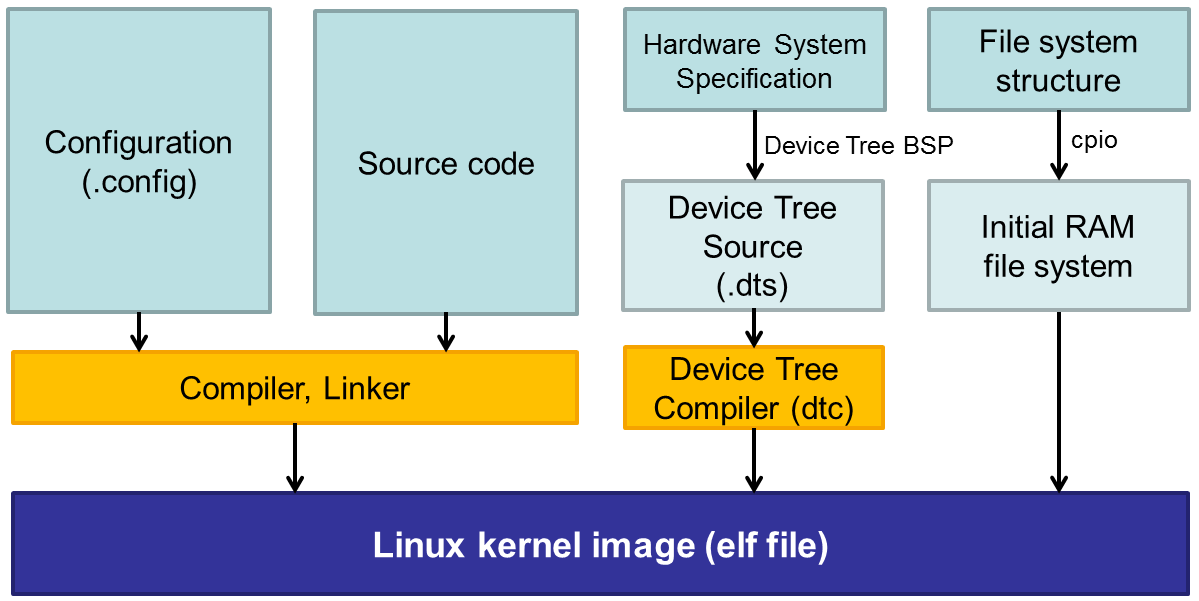
\includegraphics[width=.6\textwidth]{linux-config-build.png}
	\caption{Components of a Linux kernel build.}
%	\end{figure}
\end{wrapfigure}

Linux kernel consists of many optional sub-parts for target architectures, device drivers, special features, etc. Which of these parts are compiled and linked into the Linux kernel binary image needs to be configured in the \texttt{.config} file in the Linux kernel root directory. This file is "the configuration blueprint for building a Linux kernel image" \cite{linuxPrimer}[sec. 4.3.1] containing all (required) settings.

The \textit{MicroBlaze} processor can be configured with different feature sets (multiplier, barrel shifter, etc.). Therefore the \gls{gcc} compiler needs to be parameterized for matching the provided features of the target system \cite{mb_linux}[sec. "Kernel Configuration Details"]. These need to be set in the \texttt{XILINX\_MICROBLAZE0\_*} settings inside of the \texttt{.config} file. The \texttt{KERNEL\_BASE\_ADDR} is also an imported setting which need to match the base address of the systems main memory.

The \texttt{xps\_ll\_temac} driver is used for the Ethernet interface.

Another part of the system configuration is the \textit{Device Tree}. It is an abstraction layer for accessing hardware information, to avoid all these into assembler code \cite{device_tree}. It is accessed by the Linux kernel during the boot process for configuring itself and on lookup of hardware information. Therefore the \textit{Device Tree Source (dts)} file is compiled by the \textit{Device Tree Compiler (dtc)} during the Linux kernel build process to an \textit{Device Tree Blob (dtb)} and linked into the final Linux kernel image. It can be generated using the \textit{Device Tree Generator}, a \gls{tcl} script reading a system specification generated by \gls{xps}.

\subsection{The File System}
\label{subsec:fs}

Although possible, it makes little sense to use the Linux kernel without a file system. Therefore one of the last steps in the boot process is the initialization of a \textit{root file system (rootfs)}. \cite{linuxPrimer}[sec. 6.1] On modern desktop and server systems this \textit{rootfs} is usually just a bare minimum file system, containing all necessary files to boot the Linux kernel, mounting a file system located on a hard drive or flash memory right after booting up. But the used system in this project has no hard drive attached, neither is one required for the purpose of the project, at the moment. Therefore we will stick with the initial \textit{rootfs} as the main file system.

A simple way to provide an initial \textit{rootfs} is the \textit{Initial RAM Disk (initrd)}. This is a file system packed in a \textit{cpio} archive and linked into the Linux kernel image. It is unpacked completely into the main memory during kernel boot process. \textit{Xilinx} provides two packed file system archives for a \textit{MicroBlaze} system within their Linux kernel repository: \texttt{initramfs\_minimal.cpio.gz} and \texttt{initramfs\_complete.cpio.gz}. Both contain all files and structures sufficient for this project. The archives can be linked into the Linux kernel image by setting the configuration option \texttt{INITRAMFS\_SOURCE} to one of the file names, respectively.

\textit{cpio} archives can be unpacked using the following command. This command should be executed as privileged root user to allow the creation of node points, used in the file system.

After all changes were made to the files representing the file system, it can be packed into a \textit{cpio} archive using the bash script supplied in the appendix of this report ("\texttt{pack-fs.sh}", \ref{subsec:pack-fs}). The paths to the Linux kernel sources and file system root need to be adjusted to meet the current environment.

\section{Deployment}

The generated \textit{bitstream} of the hardware system representing the \gls{soc}, needs to be programmed into the \gls{fpga} on every power-on. This is required, because the configuration of the \gls{fpga} being set by the \textit{bitstream} is volatile. Programming the \textit{bitstream} is straight forward and can be accomplished using the \textit{Xilinx iMPACT} tool, which is part of the \textit{Xilinx ISE Design Suite}.

When the Linux kernel build is finished, the resulting \textit{\gls{elf}} file can be found at \texttt{arch/microblaze/boot/simpleImage.<dts-name>}. This file can be loaded into the \gls{fpga} using \textit{\gls{xmd}}, which is also part of the \textit{Xilinx ISE Design Suite}.

\chapter{Modifications to the system}

\section{Hardware}

Data and instructions caches were extended to 64 Kilobytes. Because it gives a slight performance gain for the system and the used \gls{fpga} had sufficient resources left.

\section{Software}

The toolchain used during the preceding project was updated to the latest version provided by \textit{Xilinx}. This version has the identifier "\texttt{microblaze-unkwnown-linux-gnu-.... (crosstool-NG 1.14.1) 4.6.2 20111018 (prerelease)}". The \gls{gcc} version included in this version is \texttt{4.6.2}. This \gls{gcc} version is not compatible with the Linux kernel version used previously. Therefore the Linux kernel was updated to version 3.5.0 (commit: \texttt{45b74487f57324fa66da40cd4d52be6f07e2aefd}\footnote{\url{http://git.xilinx.com/?p=linux-xlnx.git;a=commit;h=45b74487f57324fa66da40cd4d52be6f07e2aefd}}). The toolchain upgrade itself was required for the work on user space applications described in the following chapters.

The utilized web server software (nginx) requires the availability of an event module in the \gls{os}. Therefore \texttt{epoll} was activated in the Linux kernel configuration (\texttt{.config} file). This is done by setting the switch \texttt{CONFIG\_EPOLL=y}. Further explanations on this change can be found in the related chapter about the nginx architecture (see \ref{sec:nginx-arch}).

Another event, affecting the software part of this project was the corporate takeover of \textit{PetaLogix} by \textit{Xilinx} in late August 2012 \cite{takeover}. In consequence the efforts of both companies on Linux kernel development for the \textit{MicroBlaze} architecture were bundled, leading -- amongst others -- to a common source code repository for related developments. This alleviated the software part of the project.
\chapter{nginx}
\label{ch:nginx}

\section{Introduction}

The context of this project is to implement a testbed for a \textit{\gls{toe}} being developed in another research project. This testbed should enable testing the \gls{toe} in an environment and with workloads close to usage in real world. One usage of the \gls{tcp} is as transport layer for \gls{http} requests. \gls{http} is the second most used protocol among all internet traffic, with a share of about 20 to 30 \% (in 2008/09) \cite{internet_study} and therefore very relevant outside of lab environments. 

The server-side endpoint for \gls{http} traffic is a web server software. For this project \textit{nginx} (pronounced "engine-x") was chosen, which follows an asynchronous architecture. It was released to the public in 2004 and focuses on "high performance, high concurrency and high memory usages" \cite{aosa}. Creator and main developer of nginx is Igor Sysoev\footnote{\url{http://sysoev.ru/en/}}. During the course of this project nginx versions 1.3.4 to 1.3.10 were used.

A server system, like a web server, needs to be non-blocking to handle multiple requests at once. That is it must be able to accept and process requests while it is still busy with other, previously received requests. Systems with a "traditional" (i.e. thread-based) architecture fulfill this requirement by spawning separate processes or threads for incoming requests. An application designed by this model does not favor performance, because spawning new processes or threads "requires preparation of a new runtime environment, including allocation of heap and stack memory, and the creation of a new execution context" \cite{aosa}.

In contrast to this, \textit{nginx} was designed following an asynchronous architecture, which is accomplished by using a so called event-pattern. This means -- very much simplified -- that \textit{nginx} never "waits" during processing a request for any external operation to complete, but pushes it to an event system, being part of the \gls{os}, does something other useful like processing new requests and picks up the event, when it is finished for further processing steps.
\\

\section{Architecture}
\label{sec:nginx-arch}

The following sections provide a brief overview how \textit{nginx} and especially the event-driven architecture work.

\subsection{Overview}

A running \textit{nginx} instance always consists of atleast two processes: a \textbf{master} and a \textbf{worker} process. The master process spins-up, monitors and controls the worker processes. The worker processes handle the actual (HTTP) requests on a single thread.

\setlength{\intextsep}{0pt}
\begin{wrapfigure}[8]{r}{.4\textwidth}
	\centering
	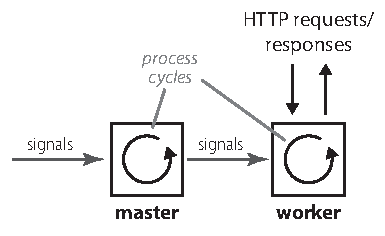
\includegraphics[scale=1]{images/nginx-overview.pdf}
	\caption{Overview of nginx process model.}
	\label{fig:nginx-overview}
\end{wrapfigure}

After initialization both processes run in a so called \textbf{process cycle}. That is an infinite loop with the process waiting to be activated from suspension by external events. For the master process these are signals send to the process which might indicate requests for shutdown, configuration reload or previously initiated timed events.

Design of the worker process had as key principle "to be as non-blocking as possible" \cite{aosa}. This is done by relying heavily on asynchronous operations being implemented through "modularity, event notifications, extensive use of callback functions and fine-tuned timers" \cite{aosa}. It also makes the process cycle of the worker process the "most complicated part of \textit{nginx}" \cite{aosa}.

Processing of requests is outsourced from the \textit{nginx} core routines to a number of dedicated modules. These modules hook into a processing pipeline forming a \textbf{chain of modules}. When a request receives, it is passed through the pipeline with every module doing the relevant work \cite{aosa}. Functionality of modules includes handling a specific protocol (e.g. \gls{http}), modifying content, filtering, handling special variables or load balancing. It is also possible to develop and integrate custom modules.

An \gls{http} request runs through a number of processing phases with dedicated \textbf{phase handlers}. These process a request and generate an appropriate response, send the header and send the body. Generation of content is done by \textbf{content handlers}. Out-of-the-box there exist several default handlers for index views or simple static files. The result of this handlers is passed to \textbf{filters} performing outbound content modifications. Filters form a separate processing pipeline, passing results among themselves until the final filter is called. Functionality of filters includes amongst others generation of header data, charset modification and gzip compression. \cite{aosa}
\\

\subsection{Event-driven Architecture}
\setlength{\intextsep}{12pt plus2pt minus2pt}
Another task of modules in the \textit{nginx} architecture is to implement functionality specific to a certain \gls{os}. One of this specifically designed tasks is the integration of an event module. Consistent and strict usage of event-driven architecture is the fundamental point of \textit{nginx}.

This is accomplished by using asynchronous, i.e. non-blocking, i/o-functions of the operating system. Handling of returning events is done through an event module provided by the \gls{os}. For this project Linux's \textit{epoll}\footnote{\url{http://linux.die.net/man/4/epoll}} module is used. \textit{epoll} handles events on file descriptors. Therefore also network related and custom events can be handled, because in Linux basically everything is a file descriptor\footnote{Linus Torvalds, "The everything-is-a-file principle": \url{http://yarchive.net/comp/linux/everything_is_file.html} (as of 12/2012)} (or process).

Events are queued and dequeued in the worker process cycle. The total workload for processing a request is split into multiple chunks, each handled after preceding, necessary operations of the \gls{os} returned.

\begin{figure}[H]
	\centering
	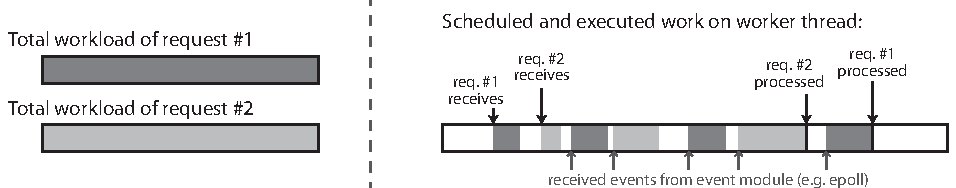
\includegraphics[scale=1]{images/nginx-event-proc.pdf}
	\caption{Processing model of worker threads.}
	\label{fig:nginx-event-proc}
\end{figure}

This leads to a responsive nginx worker thread which "can handle many thousands of concurrent connections and requests per second" \cite{aosa} (on a decent server system).

\clearpage
\section{Configuration and Building}
\label{sec:nginx-config}

After this general overview of \textit{nginx}'s architecture and underlying concepts, the next section focuses on practical implications of bringing \textit{nginx} to a \textit{MicroBlaze} system.
\\

\subsection{Extending the Configuration System}

The build process of \textit{nginx} can be configured with a number of parameters and constants to add or remove optional modules. The inclusion of modules can be configured with command line arguments to the configuration tool, but many other parameters can not be set externally.

The values of these parameters are determined by a custom "auto configuration" tool. This tool writes small C programs to a temporary file, compiles them using the configured compiler and reads back the results. By this process \textit{nginx} adjusts its own build process to the features and properties of the current system. This configuration process is not working for cross-compiling \textit{nginx} for another target system. Therefore the configuration process needed to be extended to allow input of required configuration parameters into the build process from an external source.

The implemented solution is based on a suggested patch by Daniele Salvatore Albano\footnote{\textit{Cross compilation support for nginx}, Daniele Salvatore Albano, 01/03/2011 \url{http://web.archiveorange.com/archive/v/Tuw7Ryz8rztiNaIFfqCg}}, but incorporates more of the existing parameters and is streamlined to the process of cross-compiling the Linux kernel. Cross-compiling can be enabled by setting the environment variable "\texttt{CROSS\_COMPILE}" to the suitable compiler tool chain prefix. For the \textit{MicroBlaze} tool chain this is "\texttt{microblaze-unknown-linux-gnu-}".

Parameters that are covered by this modification to the configuration system include endianness (\texttt{with-endian}), the size of primitive data types (\texttt{with-int}, \texttt{with-long}, etc.) and the maximum error number used by the \gls{os} and therefore not to be used by custom error types (\texttt{with-sys-nerr}).

To determine correct values for these introduced parameters, a small test program was written which acts in a similar way like the original nginx-auto-configuration tool (see appendix \ref{sec:nginx-env-eval}). 

Executed on the designed \gls{soc}, the program output leads to the following values:

\begin{verbatim}
    --with-endian=big \
    --with-sys-nerr=132 \
    --with-int=4 \
    --with-long=4 \
    --with-long-long=8 \
    --with-ptr-size=4 \
    --with-sig-atomic-t=4 \
    --with-size-t=4 \
    --with-off-t=4 \
    --with-time-t=4
\end{verbatim}

\subsection{Debug Mode}

By specifying \texttt{--with-debug} for configuration of \textit{nginx}. Logging and calculation of additional debug output is compiled into the resulting binary image. This is good for an initial setup and test phase, but was disabled for performance benchmarks, conducted at a later stage of the project.

\clearpage
\subsection{Modules}

\textit{nginx} consists of a number of (optional) modules. These modules can be in- or excluded from the build using parameters to the configuration tool. Objective of the \textit{nginx} build for the MicroBlaze system was a small binary with just the necessary parts included. Therefore the following modules were excluded:

\begin{verbatim}
    --without-http_rewrite_module \
    --without-http_gzip_module \
    --without-http_charset_module \
    --without-http_ssi_module \
    --without-http_userid_module \
    --without-http_access_module \
    --without-http_auth_basic_module \
    --without-http_autoindex_module \
    --without-http_status_module \
    --without-http_geo_module \
    --without-http_map_module \
    --without-http_split_clients_module \
    --without-http_referer_module \
    --without-http_proxy_module \
    --without-http_fastcgi_module \
    --without-http_uwsgi_module \
    --without-http_scgi_module \
    --without-http_memcached_module \
    --without-http_limit_conn_module \
    --without-http_limit_req_module \
    --without-http_empty_gif_module \
    --without-http_browser_module \
    --without-http_upstream_ip_hash_module \
    --without-http_upstream_least_conn_module \
    --without-http_upstream_keepalive_module \
    --without-http-cache \
    --without-pcre \
    --without-select_module \
    --without-poll_module
\end{verbatim}

Some of these modules could be included in the build, if necessary, but the modules \texttt{http\_rewrite\_module} and \texttt{http\_gzip\_module} require external libraries which are not present on the MicroBlaze system and therefore would not work.
\\

\subsection{Compiler Configuration}

Besides the configuration for \textit{nginx} itself, the compiler needs to be configured for the target \textit{MicroBlaze} system. When building the Linux kernel, the compiler configuration is set by the configuration of the kernel during the build process. \textit{nginx} does not have this functionality in its configuration system, but comes with a parameter (\texttt{--with-cc-opt=...}) to pass custom parameters to the compiler.

Through this configuration setting, the \gls{gcc} cross-compiler needs to be configured for the feature-set of the specific \textit{MicroBlaze} system. The parameters required for the developed \textit{MicroBlaze} \gls{soc} are

\texttt{-mxl-multiply-high -mno-xl-soft-mul -mno-xl-soft-div} $\hookleftarrow$ \\
\texttt{-mxl-barrel-shift -mxl-pattern-compare -mcpu=v8.30.a}

Additionally the path to the standard libraries on the system needs to be set through the \texttt{--sysroot} parameter. These libraries are part of the tool chain for \textit{MicroBlaze} systems provided by \textit{Xilinx}. 

By specifying the \texttt{--static} parameter all referenced libraries are build into the resulting binary. Therefore the binary has less dependencies for execution.

Combining it all together, the \texttt{--with-cc-opt} parameter needs to be set to the following value: 

\texttt{--with-cc-opt="-mxl-multiply-high -mno-xl-soft-mul -mno-xl-soft-div} $\hookleftarrow$ \\
\texttt{-mxl-barrel-shift -mxl-pattern-compare -mcpu=v8.30.a --static} $\hookleftarrow$ \\
\texttt{--sysroot=/home/peschuster/project/microblaze-unknown-linux-gnu/} $\hookleftarrow$ \\
\texttt{microblaze-unknown-linux-gnu/sys-root"}
\\
\\

\subsection{Memory Leaks}

One problem that arose already during very early tests were memory leaks. It turned out that \textit{nginx} allocated about 4,053.2 bytes of memory for each request. Assuming available memory of about 200 MB, \textit{nginx} crashed the complete system after approximately 50,500 requests in total. Obviously this is an unacceptable behavior for a (web) server system.

\begin{figure}[H]
\begin{minipage}{0.4\textwidth}
\begin{tabular}{|r|r|r|}
    \hline
     \textbf{requests} & \textbf{master / KB} & \textbf{worker / KB} \\
    \hline
    0     & 3064  & 3204 \\
    1000  & 3064  & 7296 \\
    2000  & 3064  & 11256 \\
    3000  & 3064  & 15348 \\
    4000  & 3064  & 19440 \\
    5000  & 3064  & 23404 \\
    6000  & 3064  & 27496 \\
    7000  & 3064  & 31588 \\
    8000  & 3064  & 35552 \\
    9000  & 3064  & 39644 \\
    10000 & 3064  & 43736 \\
    \hline
    \end{tabular}
\end{minipage}
\begin{minipage}{0.60\textwidth}
	\centering
	\begin{tikzpicture}
		\begin{axis}[width=\textwidth,height=7cm,
			xlabel={requests},
			ylabel={memory / KB},
			xmin=0,
			ymin=0,
			xmax=10000,
			extra y ticks={3064},
			%extra y tick label style={/pgf/number format/1000 sep=},
			extra y tick style={grid=major},
			extra x tick style={grid=major},
			y tick label style={/pgf/number format/1000 sep=},
			legend pos = north west]
			\addplot table[x index=0, y index=1] {graphdata/nginx-mem.csv};
			\addlegendentry{master process}
			\addplot table[x index=0, y index=2] {graphdata/nginx-mem.csv};
			\addlegendentry{worker process}
		\end{axis}
	\end{tikzpicture}
\end{minipage}
  \caption{Memory consumption of nginx processes over total requests.}
  \label{fig:nginx-mem}
\end{figure}

\subsubsection{Investigations}

The described behavior of \textit{nginx} could not be replicated on a standard x86 server system running \textit{Ubuntu Linux 12.04}. That means \textit{nginx} in general should work correct, using just as much memory as required and releasing unused memory to the \gls{os}. But this does not work properly on the \textit{MicroBlaze} system.

With activated \texttt{debug} log. \textit{nginx} writes some information about inner workings to the error log. The debug log can be activated with the following option in the \textit{nginx} runtime configuration file:

\texttt{error\_log  logs/error.log  debug;}


There must be only one \texttt{error\_log} line in the \textit{nginx} configuration file, but the option specifying the severity level is inclusive for all upper levels.

The following table shows all memory related debug messages as found in the error log for a single request to a static file on the \textit{MicroBlaze} system running an \textit{nginx} instance, which is configured as described in the previous section (sec. \ref{sec:nginx-config}):

\begin{table}[H]
\centering
\begin{tabular}{|l|l|r|r|}
    \hline
     \textbf{Log entry} & \textbf{ptr} & \textbf{allocated} & \textbf{freed} \\
    \hline \hline
\texttt{*1 malloc: 10080890:644} & 10080890 & 644 &  \\ \hline
\texttt{*1 malloc: 10080B18:1024} & 10080B18 & 1024 &  \\ \hline
\texttt{*1 posix\_memalign: 1007B5B0:4096 @16} & 1007B5B0 & 4096 &  \\ \hline \hline
\texttt{*1 free: 1007B5B0, unused: 2079} & 1007B5B0 & & 4096 \\ \hline
\texttt{*1 free: 10080890} & 10080890 & & 644 \\ \hline
\texttt{*1 free: 10080B18} & 10080B18 & & 1024 \\ \hline
\end{tabular}
\caption{Memory management related debug messages of a single request.}
\label{tab:debug_mem}
\end{table}

All pointers to allocated memory for one request are passed to the \texttt{free(..)} function of the \textit{C Standard Library} (\textit{libc}) and therefore should be released to the system. But performance and load tests on the system proved a different behavior: The \textit{nginx} worker process consumes more memory for each request with a linear relation to the number of handled requests (see figure and table \ref{fig:nginx-mem}).

Therefore it can be assumed that the error causing this misbehavior is not located in \textit{nginx} itself, but in the underlying system layers. This implies that memory management of the Linux kernel or the \textit{libc} port to the \textit{MicroBlaze} architecture are broken in the described respect. While being a strong allegation, especially because fully analyzing the problem on this wide dimensions was beyond the scope of this bachelor thesis, there are a few points promoting this theory:

\textit{Xilinx} support answer \texttt{AR \#12421} states that memory management (especially the function \texttt{free(..)}) is "very system-specific" and not fully supported and implemented for \textit{MicroBlaze} processors \cite{mbfree}. The answer was published in September 2010 and its validity is explicitly limited to versions of the \textit{MicroBlaze} processors without a hardware memory management unit. Therefore it should not apply to the used version of the \textit{MicroBlaze} processor and \textit{C Standard Library}, but it shows that these memory management functions were added to the toolchain and supporting environment only recently and might not be as stable as other, more major parts.

A possible explanation why the described, faulty behavior is only visible when using \textit{nginx}, is the unusual way \textit{nginx} deals with memory. Memory management is done by \textit{nginx}'s pool allocator. This could be seen as an abstraction to the memory allocation mechanisms provided by the \gls{os}. When another part of \textit{nginx} requires dynamically allocated memory, it requests it from the pool allocator, which itself requests a larger chunk of memory (called "pool") from the \gls{os} and distributes small blocks of the pool on requests from other parts of \textit{nginx}. When free blocks of a pool are exhausted, but none are used anymore, the complete pool is returned to the \gls{os}. \textit{nginx} uses this design to minimize system calls and reduce expensive requests for memory allocation by the hardware memory management unit \cite{aosa}. One consequence of this design is that \textit{nginx} does not reuse once allocated memory, but just allocates new memory blocks when required and releases them to the system upon finished operations. This is by design and beneficial for speed and efficiency, but comes in unfavorable, when the memory management of the system (\gls{os} and processor) might not work properly.
\\

\subsubsection{A First Workaround}

It was not possible to fix the root cause of the memory leaks during this bachelor thesis. To circumvent the described arising problems, another solution needed to be found. Otherwise practical usage of the system and extensive performance benchmarks would not be possible.

A workaround to circumvent complete system crashes during tests due to exhausted memory is to restart the \textit{nginx} worker process on low remaining system memory.

This can be accomplished by sending the \texttt{HUB} signal to the \textit{nginx} master process using the \texttt{kill} command of \textit{Unix} systems\footnote{\url{http://unixhelp.ed.ac.uk/CGI/man-cgi?kill}}. The \texttt{HUB} signal tells \textit{nginx} to reload the current configuration, resulting in spinning up new worker processes and gracefully shutting down the previous ones. This differs from complete restarts of \textit{nginx} in the way that no incoming requests are lost during the restart process.\footnote{\url{http://wiki.nginx.org/CommandLine} (as of 12/2012)}

The process id of the master process on the system is always stored in the file \texttt{/usr/local/nginx/logs/nginx.pid}. Therefore the complete command for restarting the \textit{nginx} worker process can be constructed as follows:

\texttt{kill -HUP \$( cat /usr/local/nginx/logs/nginx.pid )}

Information about currently allocated and free memory can be displayed using tools like \textit{top}\footnote{\url{http://www.busybox.net/downloads/BusyBox.html\#top}}, which provide "a view of process activity in real time" \cite{busybox}. \textit{top} internally aggregates information from multiple (virtual) file handles like e.g. \texttt{/proc/meminfo} for information about memory.
\\

\subsubsection{An Integrated Solution}

This workaround is fully functional, but requires manual actions by a user and is therefore ignorant for automation which is a key part of extensive and reproducible performance benchmarks.

An idea for an extended solution was to shift checking for low remaining memory to the \textit{nginx} master process.

After configuring and building up the system, including the start of worker processes, the master process returns to a standby mode, waiting for external signals (like the previously described \texttt{HUB} signal). This is implemented using default \textit{C Standard Library} signal implementations, mainly \texttt{sigsuspend}\footnote{\url{http://www.gnu.org/software/libc/manual/html\_node/Sigsuspend.html}}, inside of the \texttt{ngx\_master\_process\_cycle(..)} function (in the file \texttt{ngx\_worker\_cycle.c}).

A developed patch to check memory consumption of the system and initiate worker process restarts hooks in at this point inside of the master process. 

The patch consists of three major parts:

\begin{enumerate}

\item Starting a timer, to awake the master process every second from suspension. This is implemented using the Linux command \texttt{setitimer}\footnote{\url{http://linux.about.com/library/cmd/blcmdl2\_setitimer.htm}} in \texttt{ITIMER\_REAL} mode to send a \texttt{SIGALRM} signal to the current (i.e. \textit{nginx} master) process.

\item A signal handler for dealing with the \texttt{SIGALRM} signal, to check the remaining system memory and trigger a restart of worker processes, if necessary.

\item A function reading the file handle \texttt{/proc/meminfo}, parsing out the required information about free system memory and comparing it with a configured threshold value. This is implemented in the added file \texttt{ngx\_process\_memguard.c}.
\end{enumerate}

Usage of the newly implemented functionality needs to be activated upon build configuration by providing the parameter \texttt{--with-min-free-mem=[value]}. \texttt{[value]} is the threshold value in kilobytes which is compared to the free system memory to decide on a required restart of worker processes. During tests of the system this value was set to "\texttt{51200}" (kilobytes).

The complete patch is included in the appendix of this report (see \ref{appendix:memguard}) or can be found in the master branch of the \textit{nginx} fork at \url{https://github.com/peschuster/nginx}.
\\

\subsection{Compilation and Installation}

After configuration, the \textit{nginx} binary file is compiled using "\texttt{make -f objs/Makefile}". The resulting image file has a size of about 1.8 MB.

Installation into the target directory is initiated executing the command "\texttt{make install DESTDIR=<dir>}". "\texttt{<dir>}" needs to be replaced with the path to the target directory. For the environment used during this project, this is equal to the directory containing the target root file system "\texttt{/home/peschuster/project/customfs/complete}".

Executing the described \texttt{install} command creates the required directory structure with default configuration files and copies the binary image file.
\\

\subsection{Runtime Configuration}

Runtime configuration of an \textit{nginx} installation is stored in the \texttt{conf/} directory relative to the \textit{nginx} root. For this project and conducted performance tests, there was no need to change the default configuration (\texttt{nginx.conf}), which is loaded at application start up when no other options are specified.
\\

\section{Interactions with the Operating System}
\label{sec:nginx-os-if}

This section briefly describes interactions between \textit{nginx} and the underlying \gls{os} to deal with HTTP requests and responses.

User applications can interact with the network stack implemented in the Linux kernel using the \textbf{socket}\footnote{\url{http://linux.die.net/man/7/socket}} interface.
%beejs

The \textit{nginx} master process opens sockets using the \texttt{socket(..)} command. This returns a file descriptor (\texttt{int}) which is stored in the \texttt{ngx\_connection\_t} struct and used for subsequent calls to functions of the socket interface. Next the initialized socket is bind to the configured local port using \texttt{bind(..)}. This is done for all \texttt{listen} directives specified in the configuration file. The default setting "\texttt{listen 80}" opens a socket on port \texttt{80} for all IP addresses (\texttt{0.0.0.0:80}). It is also possible to listen on unix sockets by specifying a configuration value in the format "\texttt{listen unix:/tmp/nginx1.sock;}".\footnote{\url{http://nginx.org/en/docs/http/ngx\_http\_core\_module.html\#listen} (as of 12/2012)}

Last step during initialization is a call to \texttt{listen(..)} to indicate that \textit{nginx} is ready for accepting incoming connections. The \texttt{backlog} parameter, indicating the maximum number of incoming connections the \gls{os} is allowed to queue up, is set during compile time to 511. This is assumed to be a "safe value" for the Linux \gls{os}.\footnote{Mailing list answer by Igor Sysoev: \url{http://forum.nginx.org/read.php?2,9959,9967\#msg-9967}}

nginx worker processes initialize the core event module, which itself registers the callback \texttt{ngx\_event\_accept(..)} for incoming connections. Inside of \texttt{ngx\_event\_accept} the system call \texttt{accept(..)} is made. The result of \texttt{accept} calls is again a file descriptor, but just for the single, accepted connection \cite{beejs}. It is stored in a newly created struct of type \texttt{ngx\_connection\_t} for further references. Information about the remote host is also stored in this new connection struct.

Data is read from sockets using \texttt{recv(..)} which is called on parsing the HTTP request header. The call to \texttt{recv(..)} simply copies received bytes to the \texttt{header\_in} field of the current \texttt{ngx\_request\_t} struct.

Responses for requests to static files are written to the socket buffer using the two functions \texttt{writev(..)} (for HTTP header data) and \texttt{sendfile(..)} for content of the actual static file. \texttt{writev(..)} is favored over \texttt{write(..)} or \texttt{send(..)}, because it allows writing data to a file descriptor from multiple local buffers.\footnote{\url{http://linux.die.net/man/2/writev}} \textit{nginx} makes heavy usage of this extended functionality over \texttt{write(..)}. 

\texttt{sendfile(..)} is a function provided by the Linux kernel for copying data between two file descriptors. It is more efficient than a combination of \texttt{read(..)} and \texttt{write(..)}, because copying is done completely within the kernel without the requirement of "transferring data to and from user space"\footnote{http://www.kernel.org/doc/man-pages/online/pages/man2/sendfile.2.html}.

An interesting point to note is that the combined use of \texttt{writev(..)} and \texttt{sendfile(..)} leads always to atleast two TCP packets (see introduction to performance tests: section \ref{subsec:mtu}).
\chapter{Performance-Analysis}

Before going into performance tests, it is required to understand some fundamentals about network communication and the anatomy of a \gls{http} request.

\section{Introduction}

"To reduce their design complexity, most networks are organized as a \textbf{stack of layers or levels}, each one built upon the one below it" \cite{kn1}[sec. 1.3.1]. The same holds true for the protocol stack driving the "internet". There exist various models for naming and describing the different layers. In context of the internet usually the "TCP/IP Reference Model" is used \cite{kn1}. This model describes five independent layers, each build upon the next underlying layer. 

Real communication between two systems, i.e. exchange of data, always happens on the lowest layer (the "Physical Layer"). But from a logical point of view, communication happens on each layer between the two systems. Therefore each layer might add a header in front of the data, specifying meta information for its counterpart on the other system. Headers of layers above the current layer are treated as plain data, just as the actual message (see figure \ref{fig:header-layers}).

%\begin{wrapfigure}{r}{.45\textwidth}
\begin{figure}[H]
	\centering
	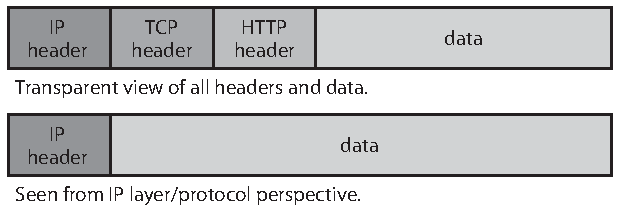
\includegraphics[scale=1]{images/protocol-headers.pdf}
	\caption{Header data for multiple protocol layers (3-5).}
	\label{fig:header-layers}
\end{figure}
%\end{wrapfigure}

Figure \ref{fig:net-layers} shows the five layers of the TCP/IP model with corresponding communication protocol and module implementing the protocol on the developed test system. When constructing performance tests this needs to be taken into account to determine for a single parameter which parts of the system are involved and might limit further improvements.

%\begin{wrapfigure}{r}{.5\textwidth}
\begin{figure}[H]
	\centering
	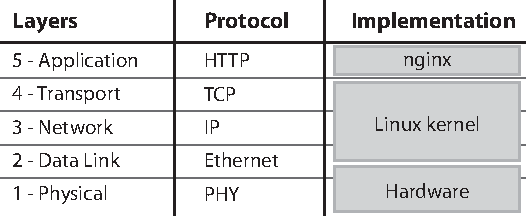
\includegraphics[scale=1]{images/network-layers.pdf}
	\caption{Layers of the network stack with reference to implementing modules.}
	\label{fig:net-layers}
\end{figure}
%\end{wrapfigure}

\subsection{Maximal Transfer Unit (MTU)}
\label{subsec:mtu}

The \gls{mtu} is the maximum size of a single unit transferred over the network in bytes. It is a parameter set for a complete network (sender, receiver, intermediate stations), specifying and limiting its capacity to a robust and reliable usage level. On differing \gls{mtu} values for connected stations the lowest takes effect. In Ethernet networks the \gls{mtu} is usually set to 1500 bytes \cite{kn1}. This includes only the data as received by the Ethernet layer. Header data of  the Ethernet protocol does not count into this size limit. When messages (including header data of upper layers) exceed the \gls{mtu} size, they are split up into multiple packets. In practice this means that for transmitting a single HTTP message (i.e. request or response) two or more \gls{tcp} messages might be required.

\subsection{Transmission Control Protocol (TCP)}

Although \gls{http} is not fixed to be used only with \gls{tcp}; \gls{http} on top of \gls{tcp} on top of \gls{ip} is the most dominant usage combination. This is, because \gls{tcp} provides reliable communication on top of unreliable networks \cite{tcp}. \gls{tcp} accomplishes this by setting up and maintaining a connection. Therefore sending data over TCP consists of three steps: establishing a connection, sending the actual message, closing the connection. To guarantee arrival of sent data, \gls{tcp} works with a handshake protocol between both involved parties. Maintaining a connection is the price to be paid for a reliable communication channel between two systems. But it also allows sending more than one messages using an already established connection. This comes in handy, when a message size exceed the \gls{mtu} or multiple \gls{http} requests are send to a server (used in persistent HTTP connections, also called "HTTP keep-alive" \cite{http}).

\gls{ip} introduced so called IP addresses as identifiers for single systems. \gls{tcp} extends this model by port numbers. An application providing services to other system (i.e. a server) uses one single port, but client applications need to open separate ports for each \gls{tcp} connection. This is required, because \gls{tcp} connections are identified by the four parts "server address", "server port", "client address" and "client port" \cite{tcp}. The TCP header contains two 16 bit fields for source and destination port \cite{kn1}. This leads to a maximum of $2^{16} = 65,536$ concurrently used (open) \gls{tcp} connections on a single client system.

\section{Measuring Web Server Performance}

Network performance is often measured as throughput in bits per second. While this gives a great insight in the capabilities of the network, there is no indication as to how many users can be served concurrently by a web server running on the system under test. To gain insights in this performance parameter, dedicated tests on \gls{http} level need to be performed.

A simple method for measuring request throughput is to "send requests to the server at a fixed rate and to measure the rate at which replies arrive" \cite{httperf}. By monotonically increasing the request rate, the server becomes saturate  at a certain point. This becomes visible in leveling off reply rates and shows that the server operates at full capacity. \cite{httperf}

\subsection{Tools}

\subsubsection{httperf}

\textit{httperf}\footnote{\url{http://www.hpl.hp.com/research/linux/httperf/}} is a tool developed at Hewlett-Packard by David Mosberger and Tai Jin to specifically measure web server performance \cite{httperf}.

\textit{httperf} has three relevant command line arguments for performing the desired performance tests: \texttt{rate}, \texttt{num-conns} and \texttt{num-calls}.

The \texttt{rate} parameter specifies the rate at which connections are created per second. \texttt{num-conns} specifies the total number of connections to be created during one test run. \texttt{num-calls} specifies the number of requests made over a single TCP connection before it is closed.

When executing \textit{httperf} a warning might be displayed:

\texttt{warning: open file limit > FD\_SETSIZE; limiting max. \# of open files to FD\_SETSIZE}

What it basically means is that the current process reached the limit of concurrently allowed open file descriptors. This is a per process limit enforced by the \gls{os}. \textit{httperf} is using the \textit{select}\footnote{"\texttt{select}" is an event library provided by the Linux kernel.} module for dealing with network tasks and creates a new file descriptor for every TCP connection. Therefore the limit on open file descriptors limits the number of TCP connections by \textit{httperf} and therefore might influence conducted performance tests.

To circumvent this issue limits on the current system need to be increased and \textit{httperf} re-compiled. This includes three steps\footnote{The described solution to the FD\_SETSIZE problem was taken from Guillaume Maury: \url{http://gom-jabbar.org/articles/2009/02/04/httperf-and-file-descriptors}.}:

\begin{enumerate}
\item The following line needs to be inserted (or updated) in \texttt{/etc/security/limits.conf}: "\texttt{* hard nofile 65535}". This increases the hard limit of open file descriptors for all users.

\item The value of the pre-compiler constant "\texttt{\_\_FD\_SET\_SIZE} needs to be increased to \texttt{65535}. It is defined in "\texttt{/usr/include/bits/typesizes.h}". (Note: This file might be located in another sub-directory, e.g. "\texttt{/usr/include/x86\_64-linux-gnu/bits/typesizes.h}".)

\item httperf needs to be re-compiled from source:\\
 \\
\texttt{wget} \url{ftp://ftp.hpl.hp.com/pub/httperf/httperf-0.9.0.tar.gz}\\
\texttt{tar xvzf httperf-0.9.0.tar.gz \&\& cd httperf-0.9.0\\
./configure \&\& make\\
sudo make install}
\end{enumerate}

A useful helper for automating test runs with increasing connection rate is \textit{autobench}\footnote{\url{http://www.xenoclast.org/autobench/}}. It is a Perl script acting as a wrapper around \textit{httperf} written by Julian Midgley.

\subsubsection{Custom Scripts}

In addition to accurate engineered test cases using \textit{httperf}, custom scripts were used to simply generate load on the server. A small Windows console application written in \texttt{C\#}, utilizing the \textit{Task Parallel Library}\footnote{\url{http://msdn.microsoft.com/de-de/library/vstudio/dd460717.aspx}} turned out to be the most efficient one with best performance characteristics.

It is also included in the appendix of this report (see \ref{appendix:csharp-load}).

\subsubsection{Wireshark}

\textit{Wireshark}\footnote{\url{http://www.wireshark.org}} is a network protocol analysis software, which captures all traffic going through a network interface. It especially helps in analyzing and inspecting captured data through deep knowledge of all common protocols.

It was used in this project for debugging initial problems with the network stack and low-level analysis of performance  test parameters.


\section{Tests}

The tests were conducted using \textit{httperf} on a virtual machine running \textit{Ubuntu Linux 12.04}. To proof that the limiting factor during the tests is not this client machine, but the system under test, all tests were also performed against a \textit{Microsoft IIS 7.5} web server instance on top of a \textit{Microsoft Windows 7 Professional} operating system running on a bare metal machine with an \textit{AMD Phenom II X4 965} processor at 3.40 GHz.

According to the \textit{HTTP Archive}\footnote{\url{http://httparchive.org/interesting.php\#responsesizes} (as of Dec. 15th 2012)} an average HTML page has a size of about 6 kB. Other content types, like images, stylesheets and script files vary on average between 5 kB and 21 kB. Therefore tests were performed using static files with two sizes: one file having exactly 10 kB (10.240 bytes) from now on referred to as "10K.html" and one very minimal HTML page having just 354 bytes ("index.html"). The major difference between these two files from a "network perspective" is that the small file can be transmitted in two TCP packets, one is used for the HTTP header and one for the actual data (see section \ref{sec:nginx-os-if}), whereas the 10 KB file needs to be split up in 9 TCP packets due to the default \gls{mtu} size of 1500 bytes. A third test run was performed requesting a file that does not exist. This results in a HTTP response with code "404 - Not Found". This is a special case, because the response is transmitted in a single TCP packet and no file needs to be read from the file system.

Figure \ref{fig:initial-req} shows request and response rates for all three test cases with an increasing connection rate (20 conn./s to 120 conn./s, step size: 10). On each connection three HTTP requests were made to the respective file. 

On every connection rate level 3,000 connections were opened to obtain reliable results. Therefore each test run included $11 \cdot 3,000 = 33,000$ connections and up to $33,000 \cdot 3 = 99,000$ requests.

\begin{figure}[H]
	\centering
	\begin{tikzpicture}
		\begin{axis}[width=\textwidth,height=7cm,
			xlabel={demanded request rate (per second)},
			ylabel={per second},
			extra y tick style={grid=major},
			extra x tick style={grid=major},
			y tick label style={/pgf/number format/1000 sep=},
			ymajorgrids=true,
			legend cell align = left,
			legend pos = north west]
			\addplot table[x index=0, y index=1] {graphdata/perf-initial3.csv};
			\addlegendentry{request (index.html)}
			\addplot table[x index=0, y index=8] {graphdata/perf-initial3.csv};
			\addlegendentry{reponse (index.html)}
			\addplot table[x index=0, y index=2] {graphdata/perf-initial3.csv};
			\addlegendentry{request (10K.html)}
			\addplot table[x index=0, y index=9] {graphdata/perf-initial3.csv};
			\addlegendentry{reponse (10K.html)}
			\addplot[color=orange,mark=diamond] table[x index=0, y index=17] {graphdata/perf-initial3.csv};
			\addlegendentry{request (404)}
			\addplot[color=teal,mark=x] table[x index=0, y index=19] {graphdata/perf-initial3.csv};
			\addlegendentry{reponse (404)}
		\end{axis}
	\end{tikzpicture}
  \caption{Request and response rates for the different test runs.}
  \label{fig:initial-req}
\end{figure}

The test result shows that at a certain request rate, the response rates levels off. For the two test runs with small response sizes, response rates even decrease slightly. At this points the server becomes saturated and requests overstep its actual capacity. These points are namely at about 300 req./s for the very small response, at about 270 req./s for the "index.html" file and at about 190 req./s for the "10K.html" file.

The difference between request and response rate origins in failed requests. The following figure shows the corresponding error rate. It increases with over-saturating the system.

\begin{figure}[H]
	\centering
	\begin{tikzpicture}
		\begin{axis}[width=\textwidth,height=6cm,
			xlabel={demanded request rate (per second)},
			ylabel={error rate (\%)},
			extra y tick style={grid=major},
			extra x tick style={grid=major},
			y tick label style={/pgf/number format/1000 sep=},
			minor tick style={very thin, gray},
			minor y tick num=3,
			ymajorgrids=true,
			legend cell align = left,
			legend pos = north west]
			\addplot table[x index=0, y index=15] {graphdata/perf-initial3.csv};
			\addlegendentry{index.html}
			\addplot table[x index=0, y index=16] {graphdata/perf-initial3.csv};
			\addlegendentry{10K.html}
			\addplot table[x index=0, y index=22] {graphdata/perf-initial3.csv};
			\addlegendentry{404}
		\end{axis}
	\end{tikzpicture}
  \caption{Error rate (failed requests) for the different test runs.}
  \label{fig:initial-req-errors}
\end{figure}

The response \textbf{rate} decreases only slowly with growing saturation, but the average response \textbf{time} increases from  5 ms to about 500-700 ms:

\begin{figure}[H]
	\centering
	\begin{tikzpicture}
		\begin{axis}[width=\textwidth,height=6cm,
			xlabel={demanded request rate (per second)},
			ylabel={response time / ms},
			extra y tick style={grid=major},
			extra x tick style={grid=major},
			y tick label style={/pgf/number format/1000 sep=},
			minor tick style={very thin, gray},
			minor y tick num=3,
			ymajorgrids=true,
			legend cell align = left,
			legend pos = north west]
			\addplot table[x index=0, y index=10] {graphdata/perf-initial3.csv};
			\addlegendentry{index.html}
			\addplot table[x index=0, y index=11] {graphdata/perf-initial3.csv};
			\addlegendentry{10K.html}
			\addplot table[x index=0, y index=20] {graphdata/perf-initial3.csv};
			\addlegendentry{404}
		\end{axis}
	\end{tikzpicture}
  \caption{Response time for the different test runs.}
  \label{fig:initial-req-time}
\end{figure}

The reason for decreasing slopes in response times might be a clogged backlog for incoming connections, resulting in an early, and therefore cheap rejection of further incoming requests.

\begin{wrapfigure}[16]{r}{.5\textwidth}
	\centering
	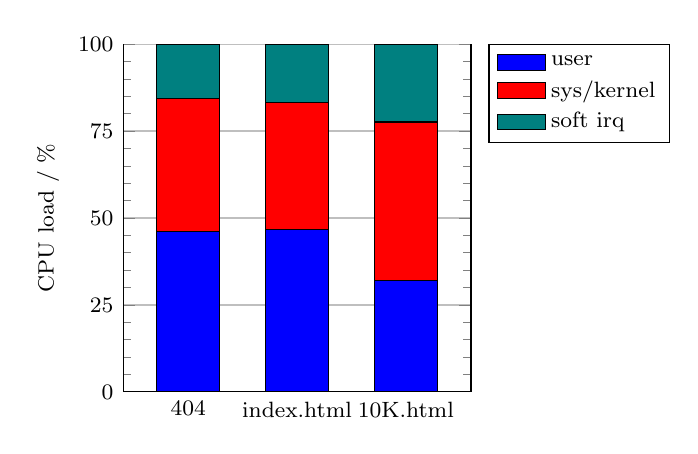
\begin{tikzpicture}
		\begin{axis}[ybar stacked,
			legend style={at={(1.05,1.0)},anchor=north west},
			xtick={0,1,2},
			axis x line*=bottom,
			tick label style={font=\footnotesize},
			legend style={font=\footnotesize},
			label style={font=\footnotesize},
			ytick={0,25,50,75,100},
			width=6cm,
			height=6cm,
			bar width=8mm,
			ylabel={CPU load / \%},
			xticklabels={404, index.html, 10K.html},
			ymajorgrids=true,
			minor tick style={very thin, gray},
			minor y tick num=4,
			ymin=0,
			ymax=100,
			area legend,
			legend cell align=left,
			enlarge x limits=0.3]
			\addplot[fill=blue] coordinates % usr
			{(0,46.2) (1,46.6) (2,32.1)};
			\addplot[fill=red] coordinates % sys
			{(0,38.1) (1,36.5) (2,45.5)};
			\addplot[fill=teal] coordinates % sirq
			{(0,15.6) (1,16.7) (2,22.3)};
			\legend{user,sys/kernel,soft irq}
		\end{axis}
	\end{tikzpicture}
	\caption{CPU load distribution for different request types.}
  \label{fig:initial-req-cpu}
\end{wrapfigure}

The difference in request and response rates the system can handle is also visible in \textbf{CPU utilization}. Main responsibility of \textit{nginx} for serving requests is to handle the HTTP part of the process. This includes parsing request headers, generating responses and delivering static files. The \gls{os} on the other hand does the "translation" to and from \gls{tcp} and handles all work on lower network layers (see also figure \ref{fig:net-layers}). An increased payload size of single responses entails therefore a shift in processing time from \textit{nginx} ("user space") towards the operations inside the Linux kernel. Figure \ref{fig:initial-req-cpu} shows exactly this correlation.

\clearpage
Network \textbf{throughput} of the tests follows naturally the trend of response rates. For tests requesting the "index.html" file and those resulting in "HTTP 404 - Not Found" responses, the shown throughput is very low, because \textit{httperf} calculates throughput using the formula $\frac{\text{[size]} \cdot \text{[total repsonses]}}{\text{[test time]}}$. Therefore very small response sizes yield a low average throughput.

\begin{figure}[H]
	\centering
	\begin{tikzpicture}
		\begin{axis}[width=\textwidth,height=6cm,
			xlabel={demanded request rate (per second)},
			ylabel={KB / s},
			extra y tick style={grid=major},
			extra x tick style={grid=major},
			y tick label style={/pgf/number format/1000 sep=},
			minor tick style={very thin, gray},
			minor y tick num=3,
			ymajorgrids=true,
			legend cell align = left,
			legend pos = north west]
			\addplot table[x index=0, y index=13] {graphdata/perf-initial3.csv};
			\addlegendentry{index.html}
			\addplot table[x index=0, y index=14] {graphdata/perf-initial3.csv};
			\addlegendentry{10K.html}
			\addplot table[x index=0, y index=21] {graphdata/perf-initial3.csv};
			\addlegendentry{404}
		\end{axis}
	\end{tikzpicture}
  \caption{Throughput for the different test runs.}
  \label{fig:initial-req-io}
\end{figure}

\subsection{Dedicated Network Throughput Tests}

To test the maximal network throughput the server can provide, a test needs to be designed focusing on just this parameter. This prevents other parts of the system from getting into the way. A constant high exchange of TCP packets can be achieved by transferring very few, but large files over the network. Therefore a large binary file having a size of 33.4 MB was used for throughput tests.

Figure \ref{fig:tcp-io-perf} shows the network throughput for requests to this file with an increasing connection rate and two HTTP requests on each connection. The system under test goes into saturation at about 61 Megabits/sec. This is equivalent to $6.1\ \%$ of the available network bandwidth, providing a maximum of 1 Gigabit/sec.

The figure also shows the total CPU utilization of the tested system.

\begin{figure}[H]
	\centering
	\begin{tikzpicture}
		\begin{axis}[width=\textwidth,height=6cm,
			xlabel={connection rate},
			ylabel={$10^6$ bits/s},
			axis  y  line*=left,
			extra y tick style={grid=major},
			extra x tick style={grid=major},
			y tick label style={/pgf/number format/1000 sep=},
			minor tick style={very thin, gray},
			minor y tick num=3,
			ymajorgrids=true,
			legend style = {at={(0.125,-.1)}, anchor=north}]
			\addplot[color=blue,mark=o] table[x index=0, y index=13] {graphdata/tcp-io-perf.csv};
			\addlegendentry{network throughput}
		\end{axis}
		\begin{axis}[width=\textwidth,height=6cm,
			ylabel={percentage},
			axis  y  line*=right,
			axis  x  line=none,
			extra y tick style={grid=major},
			extra x tick style={grid=major},
			y tick label style={/pgf/number format/1000 sep=},
			minor tick style={very thin, gray},
			minor y tick num=3,
			%ymajorgrids=true,
			legend style = {at={(0.93,-.1)}, anchor=north}]
			\addplot[color=red,mark=x] table[x index=0, y index=9] {graphdata/tcp-io-perf.csv};
			\addlegendentry{cpu load}
		\end{axis}
	\end{tikzpicture}
  \caption{Network throughput and CPU load.}
  \label{fig:tcp-io-perf}
\end{figure}

Figure \ref{fig:tcp-io-perf-cpu} shows the CPU utilization by time spent in the different types of the system. It shows that most time is spent in kernel space and handling interrupt requests by the network driver and sub system (soft irq). nginx (user space) takes only very low CPU utilization and is not the limiting factor in this test. This conforms with test results of the previous tests on smaller files.

%usr	%CPU spent by User space applications		
%sys	%CPU spent by the System (kernel mode)		
%nic	%CPU spent by Low priority user mode (nice)		
%Idle	%CPU which is available (idle)		
%io		%CPU spent by I/O waiting		
%irq	%CPU spent servicing interrupt requests		
%sirq	%CPU spent servicing soft irqs	

\begin{figure}[H]
	\centering
	\begin{tikzpicture}
		\begin{axis}[ybar stacked,width=\textwidth,height=6cm,
			xlabel={connection rate},
			ylabel={percentage},
			extra y tick style={grid=major},
			extra x tick style={grid=major},
			y tick label style={/pgf/number format/1000 sep=},
			minor tick style={very thin, gray},
			minor y tick num=3,
			ymajorgrids=true,
			bar width=10mm,
			area legend,
			legend columns=6,
			legend style = {at={(0.5,1.03)}, anchor=south}]
%			legend pos = south east]
			\addplot[fill=red] table[x index=0, y index=2] {graphdata/tcp-io-perf.csv};	%,mark=x
			\addlegendentry{user space  }
			\addplot[fill=blue] table[x index=0, y index=3] {graphdata/tcp-io-perf.csv};	%,mark=o
			\addlegendentry{system/kernel}
%			\addplot[color=magenta,mark=o] table[x index=0, y index=4] {graphdata/tcp-io-perf.csv};
%			\addlegendentry{low priority (nice)}
%			\addplot table[x index=0, y index=5] {graphdata/tcp-io-perf.csv};
%			\addlegendentry{idle}
%			\addplot[color=orange,mark=triangle] table[x index=0, y index=6] {graphdata/tcp-io-perf.csv};
%			\addlegendentry{io (waiting)}
%			\addplot[color=green,mark=|] table[x index=0, y index=7] {graphdata/tcp-io-perf.csv};
%			\addlegendentry{irq}
			\addplot[fill=teal] table[x index=0, y index=8] {graphdata/tcp-io-perf.csv};	%,mark=diamond
			\addlegendentry{soft irq}
		\end{axis}
	\end{tikzpicture}
  \caption{CPU utilization by category.}
  \label{fig:tcp-io-perf-cpu}
\end{figure}

To proof that obtained performance limits were not limits of the client executing the tests or the network infrastructure, the same test was executed against a "reference system" running an \textit{Microsoft IIS 7.5} web server. Figure \ref{fig:tcp-io-perf-iis} shows the results. Measured throughput (averaged per request) had a maximum at about 515.7 Megabits/sec which outplays the results of the \textit{MicroBlaze} system by more than a factor of eight.

\begin{figure}[H]
	\centering
	\begin{tikzpicture}
		\begin{axis}[width=\textwidth,height=6cm,
			xlabel={connection rate},
			ylabel={$10^6$ bits/s},
			extra y tick style={grid=major},
			extra x tick style={grid=major},
			y tick label style={/pgf/number format/1000 sep=},
			minor tick style={very thin, gray},
			minor y tick num=3,
			ymajorgrids=true,
			legend pos = south east]
			\addplot table[x index=0, y index=15] {graphdata/tcp-io-perf.csv};
			\addlegendentry{network throughput}
		\end{axis}
	\end{tikzpicture}
  \caption{Network throughput of an AMD Phenom II X4 processor at 3.40 GHz running Microsoft IIS 7.5 on Windows 7.}
  \label{fig:tcp-io-perf-iis}
\end{figure}

\section{Discussion of Results}

Obtained performance results show that the designed System on Chip with custom configured and compiled Linux kernel is capable of running a web server serving up to about 300 requests per second and 100 concurrent connections. Compared to the low performance indicator of 48.94 BogoMIPS\footnote{"The number of million times per second a processor can do absolutely nothing." (untraceable source: Eric S Raymond, Geoff Mackenzie -- \url{http://www.tldp.org/HOWTO/html\_single/BogoMips/})}, which is less than a $\frac{1}{130}$ of the value Linux kernel reports for a virtualized \textit{AMD Phenom II X4} processor at 3.40 GHz running on two cores\footnote{6414.98 BogoMips}, this is not to bad. But the capacity of the server would not be sufficient for running it as a public web server connected to the global internet infrastructure. Especially because response rates rapidly decrease with increasing byte size of responses, because of a larger amount of TCP packets required for transmitting the response.

A reduction in the number of TCP packets could be achieved by using so called "Jumbo Frames". These are Ethernet frames with a data size larger than the default \gls{mtu} of 1500 bytes. The required setting can be configured executing the command "\texttt{ifconfig eth0 mtu [new size]}". Where \texttt{[new size]} is the new \gls{mtu} size in bytes. Unfortunately this does not seem to be fully supported by the \textit{Xilinx LL TEMAC} Ethernet driver\footnote{see Xilinx forum: \url{http://forums.xilinx.com/t5/Embedded-Linux/Jumbo-frames-ifconfig-crash-and-xps-ll-temac-issues/td-p/211911} (as of 12/2012)}, leading to TCP packets with a total size larger than 1500 bytes to be corrupted and therefore lost "on the network". Besides this, Jumbo Frames would have to be supported on the client and all intermediate stations as well, which can not be guaranteed on a public network or service.

\textit{nginx} provides a configuration setting "\texttt{worker\_connections}" which limits the maximum amount of concurrently handled connections by a worker process. During tests this setting had a value of 768. But neither changing the number of maximum allowed connection to 1024 nor 512 had any influence in observed response rates. Therefore it is save to be assumed that no internal limit for concurrent connections affected the test results. But therefore this part does not have any room for improvements, either.

Especially the tests for maximum network throughput showed that the main bottleneck is in the TCP/network stack on the test system. Besides providing more processing power to the system, optimizing this part of the Linux kernel is hardly possible in the project context. Another option would be to offload processing of TCP connections, requests and responses to dedicated hardware circuitry, implemented as a network interface with enhanced functionality. This possible solution is also refereed to by the title of this thesis using the word "accelerated", but requires deep integration into already available functions of the operating system. Therefore the next two chapters will focus on giving an overview of the Linux network stack and possible integration options for a TCP Offload Engine (TOE).
\chapter{Linux Network Stack}

\section{Overview}

\begin{wrapfigure}[20]{r}{.35\textwidth}
	\centering
	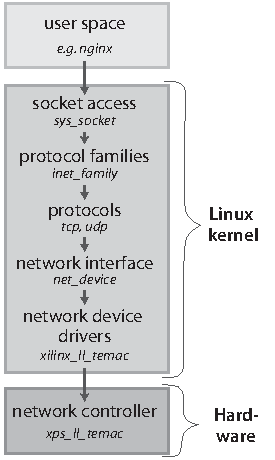
\includegraphics[scale=1]{images/net-stack.pdf}
	\caption{Linux network stack.}
	\label{fig:net-stack}
\end{wrapfigure}
The top most layer of the Linux network stack is the \textbf{system call interface} to create and operate on sockets \cite{netstackana}. The usage of this interface by \textit{nginx} was already described in section \ref{sec:nginx-os-if}. Its purpose is to multiplex networking calls by the user into the kernel \cite{netstackana}. Once a file descriptor was created using the socket interface, data can be exchanged with the network system though general operations on file descriptors like \textit{write} and \textit{read}, too. The socket interface is completely agnostic to different protocols or implementations by network devices and drivers. Its main underlying structure is \texttt{struct sock}, containing all relevant information about a specific socket, like available functions and protocol specific state information.\footnote{\url{http://www.ecsl.cs.sunysb.edu/elibrary/linux/network/LinuxKernel.pdf}} Thereby also protocol and implementation specific functionality is bind to a socket using function pointers (as defined in \texttt{struct inet\_protosw}) \cite{netstackana}.

Whereas the more general data structure \texttt{struct sock} contains mainly meta information about a socket, the major structure for storing data is \texttt{struct sk\_buff}. \textbf{\texttt{sk\_buff}} contains packet data and state information. It is used for to be sent, as well as for received packets almost through out all layers of the network stack. \cite{netstackana}

The gap between protocol handling and device drivers is bridged by the \textbf{network interface} (\textit{netif}) layer. This is a hardware device "agnostic interface layer" \cite{netstackana} with the major purpose of connecting protocols to hardware devices. Information about devices is provided through the \texttt{struct net\_device}. On system start-up all available devices provide register them selves with a filled out \texttt{net\_device} structure. From there on they are know to the network interface layer.

The lowest layer of the network stack being part of the Linux kernel is build by \textbf{device drivers}. These hook into the network interface layer and manage physical/hardware network controllers. For the implemented System on Chip this is the \texttt{xps\_ll\_temac} \gls{ip} core.

Since introduction of the "New API" (NAPI) for communication between device drivers processing packets and the network interface layer, most of the workload for received and to be sent packets is scheduled through software interrupt requests (also known as \textit{soft irq} or \textit{sirq}).\footnote{\url{http://www.linuxfoundation.org/collaborate/workgroups/networking/napi} (as of 12/2012)} During performance tests described in the previous chapter this was visible through high CPU utilization of the \textit{sirq} category.

The network interface layer enqueues \texttt{sk\_buff} packets for transmission using the function \texttt{hard\_start\_xmit(..)}. The device driver pushes received packets to the upper layer using \texttt{netif\_receive\_skb(..)}. \cite{netstackana}
\chapter{Conclusion}

\section{Project Review}

I chose this project, because it promised to cover many topics of personal interest, including network systems, performance oriented research and optimization, web technology and System on chip design. In retrospective these expectations were fulfilled, but came with a steep learning curve.

After some weeks of administrative problems concerning setup of the environment and required tools, the project could get started. The following two to three weeks were filled with learning the utilized tools and understanding the overall process of designing an \gls{ip} core based \gls{soc} on a \gls{fpga}. When being familiar with the general concepts and topics covered by this project, I started to focus on the actual project goal, assembled a time schedule and defined an, from my point of view at that time, doable intermediate goal for the project seminar. But as it turned out during the course of the project, it was hardly possible to stick to the schedule and the planned outcome of the project seminar. This was mainly reasoned in lots of problems occurring at points, which initially seemed to be straight forward implementation tasks, but in fact contained many non-trivial pitfalls. 

One of the major difficulties solved during this project seminar was the fact that there exists some documentation and reference projects (partly) covering the project objective, on the one hand, but these could not be ported easily to the tools and hardware family used in this project. This was especially a problem, because \textit{Xilinx} makes little effort to keep new versions of their tools and included \gls{ip} cores compatible with older hardware families. Discovering and keeping this circumstance in mind, was one of the key points in successfully implementing the described outcome of the project seminar.

All in all working through this project seminar was a hard but valuable experience, especially learning about all the interfaces and dependencies between the different levels in the stack of a computer system.

The project seminar covered only the first part of the project goal. So there is naturally some work to be done to finish the project. This covers especially everything around incorporating custom user space applications (like \textit{nginx}) and an accurate measurement and evaluation of performance parameters of the designed system.

Besides these outstanding topics, improvements to already implemented parts of the system could be made, too. To name a few, the baud rate of the serial \gls{ip} core could be increased to enable a more responsive console interface for accessing the system. An additional, non-volatile file system could be added to the system to circumvent the need for programming a complete image onto the \gls{fpga} on every persisted change to the file system. This could be done by including a \textit{Network File System (NFS)} or a file system stored on a flash drive.

When the complete system is implemented, including the event-based server, as stated in the project title, the focus of the project work needs to be shifted more towards measuring the performance parameters of the system. As part of this work an "\textit{TCP Offload Engine}", designed in a parallel project could be incorporated into the system. Purpose of this offload engine is to fork processing load resulting from incoming and outgoing network traffic from the \gls{cpu} to a designated hardware core. It is expected that this will speed up the overall performance of the system, allowing either the usage of less hardware resources or a higher network throughput.

The next steps in a subsequent project seminar or bachelor thesis would be to get  cross compilation of user space applications working, incorporate \textit{nginx} into the system and conduct the mentioned performance measurements.


\section{Evaluation}
\appendix 

\chapter{Hardware Project Configurations}

\section{Microprocessor Hardware Specification}

\begin{verbatim}
# ##############################################################################
# Created by Base System Builder Wizard for Xilinx EDK 14.1 Build EDK_P.15xf
# Tue Aug 07 16:08:53 2012
# Target Board:  Xilinx XUPV5-LX110T Evaluation Platform Rev A
# Family:    virtex5
# Device:    xc5vlx110t
# Package:   ff1136
# Speed Grade:  -1
# Processor number: 1
# Processor 1: microblaze_0
# System clock frequency: 100.0
# Debug Interface: On-Chip HW Debug Module
# ##############################################################################
 PARAMETER VERSION = 2.1.0


 PORT fpga_0_RS232_Uart_1_RX_pin = fpga_0_RS232_Uart_1_RX_pin, DIR = I
 PORT fpga_0_RS232_Uart_1_TX_pin = fpga_0_RS232_Uart_1_TX_pin, DIR = O
 PORT fpga_0_LEDs_8Bit_GPIO_IO_pin = fpga_0_LEDs_8Bit_GPIO_IO_pin, DIR = IO, VEC = [0:7]
 PORT fpga_0_LEDs_Positions_GPIO_IO_pin = fpga_0_LEDs_Positions_GPIO_IO_pin, DIR = IO, VEC = [0:4]
 PORT fpga_0_Push_Buttons_5Bit_GPIO_IO_pin = fpga_0_Push_Buttons_5Bit_GPIO_IO_pin, DIR = IO, VEC = [0:4]
 PORT fpga_0_DIP_Switches_8Bit_GPIO_IO_pin = fpga_0_DIP_Switches_8Bit_GPIO_IO_pin, DIR = IO, VEC = [0:7]
 PORT fpga_0_IIC_EEPROM_Sda_pin = fpga_0_IIC_EEPROM_Sda_pin, DIR = IO
 PORT fpga_0_IIC_EEPROM_Scl_pin = fpga_0_IIC_EEPROM_Scl_pin, DIR = IO
 PORT fpga_0_DDR2_SDRAM_DDR2_Clk_pin = fpga_0_DDR2_SDRAM_DDR2_Clk_pin, DIR = O, VEC = [1:0]
 PORT fpga_0_DDR2_SDRAM_DDR2_Clk_n_pin = fpga_0_DDR2_SDRAM_DDR2_Clk_n_pin, DIR = O, VEC = [1:0]
 PORT fpga_0_DDR2_SDRAM_DDR2_CE_pin = fpga_0_DDR2_SDRAM_DDR2_CE_pin, DIR = O, VEC = [1:0]
 PORT fpga_0_DDR2_SDRAM_DDR2_CS_n_pin = fpga_0_DDR2_SDRAM_DDR2_CS_n_pin, DIR = O, VEC = [1:0]
 PORT fpga_0_DDR2_SDRAM_DDR2_ODT_pin = fpga_0_DDR2_SDRAM_DDR2_ODT_pin, DIR = O, VEC = [1:0]
 PORT fpga_0_DDR2_SDRAM_DDR2_RAS_n_pin = fpga_0_DDR2_SDRAM_DDR2_RAS_n_pin, DIR = O
 PORT fpga_0_DDR2_SDRAM_DDR2_CAS_n_pin = fpga_0_DDR2_SDRAM_DDR2_CAS_n_pin, DIR = O
 PORT fpga_0_DDR2_SDRAM_DDR2_WE_n_pin = fpga_0_DDR2_SDRAM_DDR2_WE_n_pin, DIR = O
 PORT fpga_0_DDR2_SDRAM_DDR2_BankAddr_pin = fpga_0_DDR2_SDRAM_DDR2_BankAddr_pin, DIR = O, VEC = [1:0]
 PORT fpga_0_DDR2_SDRAM_DDR2_Addr_pin = fpga_0_DDR2_SDRAM_DDR2_Addr_pin, DIR = O, VEC = [12:0]
 PORT fpga_0_DDR2_SDRAM_DDR2_DQ_pin = fpga_0_DDR2_SDRAM_DDR2_DQ_pin, DIR = IO, VEC = [63:0]
 PORT fpga_0_DDR2_SDRAM_DDR2_DM_pin = fpga_0_DDR2_SDRAM_DDR2_DM_pin, DIR = O, VEC = [7:0]
 PORT fpga_0_DDR2_SDRAM_DDR2_DQS_pin = fpga_0_DDR2_SDRAM_DDR2_DQS_pin, DIR = IO, VEC = [7:0]
 PORT fpga_0_DDR2_SDRAM_DDR2_DQS_n_pin = fpga_0_DDR2_SDRAM_DDR2_DQS_n_pin, DIR = IO, VEC = [7:0]
 PORT fpga_0_Hard_Ethernet_MAC_TemacPhy_RST_n_pin = fpga_0_Hard_Ethernet_MAC_TemacPhy_RST_n_pin, DIR = O
 PORT fpga_0_Hard_Ethernet_MAC_MII_TX_CLK_0_pin = fpga_0_Hard_Ethernet_MAC_MII_TX_CLK_0_pin, DIR = I
 PORT fpga_0_Hard_Ethernet_MAC_GMII_TXD_0_pin = fpga_0_Hard_Ethernet_MAC_GMII_TXD_0_pin, DIR = O, VEC = [7:0]
 PORT fpga_0_Hard_Ethernet_MAC_GMII_TX_EN_0_pin = fpga_0_Hard_Ethernet_MAC_GMII_TX_EN_0_pin, DIR = O
 PORT fpga_0_Hard_Ethernet_MAC_GMII_TX_ER_0_pin = fpga_0_Hard_Ethernet_MAC_GMII_TX_ER_0_pin, DIR = O
 PORT fpga_0_Hard_Ethernet_MAC_GMII_TX_CLK_0_pin = fpga_0_Hard_Ethernet_MAC_GMII_TX_CLK_0_pin, DIR = O
 PORT fpga_0_Hard_Ethernet_MAC_GMII_RXD_0_pin = fpga_0_Hard_Ethernet_MAC_GMII_RXD_0_pin, DIR = I, VEC = [7:0]
 PORT fpga_0_Hard_Ethernet_MAC_GMII_RX_DV_0_pin = fpga_0_Hard_Ethernet_MAC_GMII_RX_DV_0_pin, DIR = I
 PORT fpga_0_Hard_Ethernet_MAC_GMII_RX_ER_0_pin = fpga_0_Hard_Ethernet_MAC_GMII_RX_ER_0_pin, DIR = I
 PORT fpga_0_Hard_Ethernet_MAC_GMII_RX_CLK_0_pin = fpga_0_Hard_Ethernet_MAC_GMII_RX_CLK_0_pin, DIR = I
 PORT fpga_0_Hard_Ethernet_MAC_MDC_0_pin = fpga_0_Hard_Ethernet_MAC_MDC_0_pin, DIR = O
 PORT fpga_0_Hard_Ethernet_MAC_MDIO_0_pin = fpga_0_Hard_Ethernet_MAC_MDIO_0_pin, DIR = IO
 PORT fpga_0_Hard_Ethernet_MAC_PHY_MII_INT_pin = fpga_0_Hard_Ethernet_MAC_PHY_MII_INT_pin, DIR = I, SIGIS = INTERRUPT, SENSITIVITY = LEVEL_LOW, INTERRUPT_PRIORITY = MEDIUM
 PORT fpga_0_clk_1_sys_clk_pin = CLK_S, DIR = I, SIGIS = CLK, CLK_FREQ = 100000000
 PORT fpga_0_rst_1_sys_rst_pin = sys_rst_s, DIR = I, SIGIS = RST, RST_POLARITY = 0


BEGIN microblaze
 PARAMETER INSTANCE = microblaze_0
 PARAMETER C_USE_BARREL = 1
 PARAMETER C_DEBUG_ENABLED = 1
 PARAMETER C_ICACHE_BASEADDR = 0x50000000
 PARAMETER C_ICACHE_HIGHADDR = 0x5fffffff
 PARAMETER C_CACHE_BYTE_SIZE = 16384
 PARAMETER C_ICACHE_ALWAYS_USED = 1
 PARAMETER C_ICACHE_LINE_LEN = 8
 PARAMETER C_ICACHE_STREAMS = 1
 PARAMETER C_ICACHE_VICTIMS = 8
 PARAMETER C_DCACHE_BASEADDR = 0x50000000
 PARAMETER C_DCACHE_HIGHADDR = 0x5fffffff
 PARAMETER C_DCACHE_BYTE_SIZE = 16384
 PARAMETER C_DCACHE_ALWAYS_USED = 1
 PARAMETER HW_VER = 8.30.a
 PARAMETER C_USE_ICACHE = 1
 PARAMETER C_USE_DCACHE = 1
 PARAMETER C_PVR = 2
 PARAMETER C_USE_MMU = 3
 PARAMETER C_MMU_ZONES = 2
 PARAMETER C_USE_HW_MUL = 2
 PARAMETER C_USE_DIV = 1
 BUS_INTERFACE DLMB = dlmb
 BUS_INTERFACE ILMB = ilmb
 BUS_INTERFACE DPLB = mb_plb
 BUS_INTERFACE IPLB = mb_plb
 BUS_INTERFACE DXCL = microblaze_0_DXCL
 BUS_INTERFACE IXCL = microblaze_0_IXCL
 BUS_INTERFACE DEBUG = microblaze_0_mdm_bus
 PORT MB_RESET = mb_reset
 PORT INTERRUPT = microblaze_0_Interrupt
END

BEGIN plb_v46
 PARAMETER INSTANCE = mb_plb
 PARAMETER HW_VER = 1.05.a
 PORT PLB_Clk = clk_100_0000MHzPLL0
 PORT SYS_Rst = sys_bus_reset
END

BEGIN lmb_v10
 PARAMETER INSTANCE = ilmb
 PARAMETER HW_VER = 2.00.b
 PORT LMB_Clk = clk_100_0000MHzPLL0
 PORT SYS_Rst = sys_bus_reset
END

BEGIN lmb_v10
 PARAMETER INSTANCE = dlmb
 PARAMETER HW_VER = 2.00.b
 PORT LMB_Clk = clk_100_0000MHzPLL0
 PORT SYS_Rst = sys_bus_reset
END

BEGIN lmb_bram_if_cntlr
 PARAMETER INSTANCE = dlmb_cntlr
 PARAMETER HW_VER = 3.00.b
 PARAMETER C_BASEADDR = 0x00000000
 PARAMETER C_HIGHADDR = 0x0000ffff
 BUS_INTERFACE SLMB = dlmb
 BUS_INTERFACE BRAM_PORT = dlmb_port
END

BEGIN lmb_bram_if_cntlr
 PARAMETER INSTANCE = ilmb_cntlr
 PARAMETER HW_VER = 3.00.b
 PARAMETER C_BASEADDR = 0x00000000
 PARAMETER C_HIGHADDR = 0x0000ffff
 BUS_INTERFACE SLMB = ilmb
 BUS_INTERFACE BRAM_PORT = ilmb_port
END

BEGIN bram_block
 PARAMETER INSTANCE = lmb_bram
 PARAMETER HW_VER = 1.00.a
 BUS_INTERFACE PORTA = ilmb_port
 BUS_INTERFACE PORTB = dlmb_port
END

BEGIN xps_uartlite
 PARAMETER INSTANCE = RS232_Uart_1
 PARAMETER C_BAUDRATE = 9600
 PARAMETER C_DATA_BITS = 8
 PARAMETER C_USE_PARITY = 0
 PARAMETER C_ODD_PARITY = 0
 PARAMETER HW_VER = 1.02.a
 PARAMETER C_BASEADDR = 0x84020000
 PARAMETER C_HIGHADDR = 0x8402ffff
 BUS_INTERFACE SPLB = mb_plb
 PORT RX = fpga_0_RS232_Uart_1_RX_pin
 PORT TX = fpga_0_RS232_Uart_1_TX_pin
 PORT Interrupt = RS232_Uart_1_Interrupt
END

BEGIN xps_gpio
 PARAMETER INSTANCE = LEDs_8Bit
 PARAMETER C_ALL_INPUTS = 0
 PARAMETER C_GPIO_WIDTH = 8
 PARAMETER C_INTERRUPT_PRESENT = 0
 PARAMETER C_IS_DUAL = 0
 PARAMETER HW_VER = 2.00.a
 PARAMETER C_BASEADDR = 0x81440000
 PARAMETER C_HIGHADDR = 0x8144ffff
 BUS_INTERFACE SPLB = mb_plb
 PORT GPIO_IO = fpga_0_LEDs_8Bit_GPIO_IO_pin
END

BEGIN xps_gpio
 PARAMETER INSTANCE = LEDs_Positions
 PARAMETER C_ALL_INPUTS = 0
 PARAMETER C_GPIO_WIDTH = 5
 PARAMETER C_INTERRUPT_PRESENT = 0
 PARAMETER C_IS_DUAL = 0
 PARAMETER HW_VER = 2.00.a
 PARAMETER C_BASEADDR = 0x81420000
 PARAMETER C_HIGHADDR = 0x8142ffff
 BUS_INTERFACE SPLB = mb_plb
 PORT GPIO_IO = fpga_0_LEDs_Positions_GPIO_IO_pin
END

BEGIN xps_gpio
 PARAMETER INSTANCE = Push_Buttons_5Bit
 PARAMETER C_ALL_INPUTS = 1
 PARAMETER C_GPIO_WIDTH = 5
 PARAMETER C_INTERRUPT_PRESENT = 0
 PARAMETER C_IS_DUAL = 0
 PARAMETER HW_VER = 2.00.a
 PARAMETER C_BASEADDR = 0x81400000
 PARAMETER C_HIGHADDR = 0x8140ffff
 BUS_INTERFACE SPLB = mb_plb
 PORT GPIO_IO = fpga_0_Push_Buttons_5Bit_GPIO_IO_pin
END

BEGIN xps_gpio
 PARAMETER INSTANCE = DIP_Switches_8Bit
 PARAMETER C_ALL_INPUTS = 1
 PARAMETER C_GPIO_WIDTH = 8
 PARAMETER C_INTERRUPT_PRESENT = 0
 PARAMETER C_IS_DUAL = 0
 PARAMETER HW_VER = 2.00.a
 PARAMETER C_BASEADDR = 0x81460000
 PARAMETER C_HIGHADDR = 0x8146ffff
 BUS_INTERFACE SPLB = mb_plb
 PORT GPIO_IO = fpga_0_DIP_Switches_8Bit_GPIO_IO_pin
END

BEGIN xps_iic
 PARAMETER INSTANCE = IIC_EEPROM
 PARAMETER C_IIC_FREQ = 100000
 PARAMETER C_TEN_BIT_ADR = 0
 PARAMETER HW_VER = 2.03.a
 PARAMETER C_BASEADDR = 0x81600000
 PARAMETER C_HIGHADDR = 0x8160ffff
 BUS_INTERFACE SPLB = mb_plb
 PORT IIC2INTC_Irpt = IIC_EEPROM_IIC2INTC_Irpt
 PORT Sda = fpga_0_IIC_EEPROM_Sda_pin
 PORT Scl = fpga_0_IIC_EEPROM_Scl_pin
END

BEGIN mpmc
 PARAMETER INSTANCE = DDR2_SDRAM
 PARAMETER C_NUM_PORTS = 3
 PARAMETER C_NUM_IDELAYCTRL = 3
 PARAMETER C_IDELAYCTRL_LOC = IDELAYCTRL_X0Y5-IDELAYCTRL_X0Y1-IDELAYCTRL_X0Y0
 PARAMETER C_MEM_PARTNO = MT4HTF3264H-667
 PARAMETER C_MEM_ODT_TYPE = 1
 PARAMETER C_MEM_CLK_WIDTH = 2
 PARAMETER C_MEM_ODT_WIDTH = 2
 PARAMETER C_MEM_CE_WIDTH = 2
 PARAMETER C_MEM_CS_N_WIDTH = 2
 PARAMETER C_DDR2_DQSN_ENABLE = 1
 PARAMETER C_PIM0_BASETYPE = 1
 PARAMETER C_PIM1_BASETYPE = 1
 PARAMETER C_PIM2_BASETYPE = 3
 PARAMETER C_SDMA2_PI2LL_CLK_RATIO = 2
 PARAMETER HW_VER = 6.05.a
 PARAMETER C_MPMC_BASEADDR = 0x50000000
 PARAMETER C_MPMC_HIGHADDR = 0x5FFFFFFF
 PARAMETER C_SDMA_CTRL_BASEADDR = 0x84600000
 PARAMETER C_SDMA_CTRL_HIGHADDR = 0x8460FFFF
 BUS_INTERFACE XCL0 = microblaze_0_IXCL
 BUS_INTERFACE XCL1 = microblaze_0_DXCL
 BUS_INTERFACE SDMA_CTRL2 = mb_plb
 BUS_INTERFACE SDMA_LL2 = Hard_Ethernet_MAC_LLINK0
 PORT SDMA2_Clk = clk_100_0000MHzPLL0
 PORT SDMA2_Rx_IntOut = DDR2_SDRAM_SDMA2_Rx_IntOut
 PORT SDMA2_Tx_IntOut = DDR2_SDRAM_SDMA2_Tx_IntOut
 PORT MPMC_Clk0 = clk_200_0000MHzPLL0
 PORT MPMC_Clk0_DIV2 = clk_100_0000MHzPLL0
 PORT MPMC_Clk90 = clk_200_0000MHz90PLL0
 PORT MPMC_Clk_200MHz = clk_200_0000MHzPLL0
 PORT MPMC_Rst = sys_periph_reset
 PORT DDR2_Clk = fpga_0_DDR2_SDRAM_DDR2_Clk_pin
 PORT DDR2_Clk_n = fpga_0_DDR2_SDRAM_DDR2_Clk_n_pin
 PORT DDR2_CE = fpga_0_DDR2_SDRAM_DDR2_CE_pin
 PORT DDR2_CS_n = fpga_0_DDR2_SDRAM_DDR2_CS_n_pin
 PORT DDR2_ODT = fpga_0_DDR2_SDRAM_DDR2_ODT_pin
 PORT DDR2_RAS_n = fpga_0_DDR2_SDRAM_DDR2_RAS_n_pin
 PORT DDR2_CAS_n = fpga_0_DDR2_SDRAM_DDR2_CAS_n_pin
 PORT DDR2_WE_n = fpga_0_DDR2_SDRAM_DDR2_WE_n_pin
 PORT DDR2_BankAddr = fpga_0_DDR2_SDRAM_DDR2_BankAddr_pin
 PORT DDR2_Addr = fpga_0_DDR2_SDRAM_DDR2_Addr_pin
 PORT DDR2_DQ = fpga_0_DDR2_SDRAM_DDR2_DQ_pin
 PORT DDR2_DM = fpga_0_DDR2_SDRAM_DDR2_DM_pin
 PORT DDR2_DQS = fpga_0_DDR2_SDRAM_DDR2_DQS_pin
 PORT DDR2_DQS_n = fpga_0_DDR2_SDRAM_DDR2_DQS_n_pin
END

BEGIN xps_ll_temac
 PARAMETER INSTANCE = Hard_Ethernet_MAC
 PARAMETER C_NUM_IDELAYCTRL = 2
 PARAMETER C_IDELAYCTRL_LOC = IDELAYCTRL_X0Y4-IDELAYCTRL_X1Y5
 PARAMETER C_FAMILY = virtex5
 PARAMETER C_PHY_TYPE = 1
 PARAMETER C_TEMAC1_ENABLED = 0
 PARAMETER C_BUS2CORE_CLK_RATIO = 1
 PARAMETER C_TEMAC_TYPE = 0
 PARAMETER C_TEMAC0_PHYADDR = 0b00001
 PARAMETER HW_VER = 2.03.a
 PARAMETER C_BASEADDR = 0x87000000
 PARAMETER C_HIGHADDR = 0x8707ffff
 PARAMETER C_TEMAC0_TXCSUM = 1
 PARAMETER C_TEMAC0_RXCSUM = 1
 BUS_INTERFACE SPLB = mb_plb
 BUS_INTERFACE LLINK0 = Hard_Ethernet_MAC_LLINK0
 PORT TemacIntc0_Irpt = Hard_Ethernet_MAC_TemacIntc0_Irpt
 PORT TemacPhy_RST_n = fpga_0_Hard_Ethernet_MAC_TemacPhy_RST_n_pin
 PORT GTX_CLK_0 = clk_125_0000MHz
 PORT REFCLK = clk_200_0000MHzPLL0
 PORT LlinkTemac0_CLK = clk_100_0000MHzPLL0
 PORT MII_TX_CLK_0 = fpga_0_Hard_Ethernet_MAC_MII_TX_CLK_0_pin
 PORT GMII_TXD_0 = fpga_0_Hard_Ethernet_MAC_GMII_TXD_0_pin
 PORT GMII_TX_EN_0 = fpga_0_Hard_Ethernet_MAC_GMII_TX_EN_0_pin
 PORT GMII_TX_ER_0 = fpga_0_Hard_Ethernet_MAC_GMII_TX_ER_0_pin
 PORT GMII_TX_CLK_0 = fpga_0_Hard_Ethernet_MAC_GMII_TX_CLK_0_pin
 PORT GMII_RXD_0 = fpga_0_Hard_Ethernet_MAC_GMII_RXD_0_pin
 PORT GMII_RX_DV_0 = fpga_0_Hard_Ethernet_MAC_GMII_RX_DV_0_pin
 PORT GMII_RX_ER_0 = fpga_0_Hard_Ethernet_MAC_GMII_RX_ER_0_pin
 PORT GMII_RX_CLK_0 = fpga_0_Hard_Ethernet_MAC_GMII_RX_CLK_0_pin
 PORT MDC_0 = fpga_0_Hard_Ethernet_MAC_MDC_0_pin
 PORT MDIO_0 = fpga_0_Hard_Ethernet_MAC_MDIO_0_pin
END

BEGIN xps_timer
 PARAMETER INSTANCE = xps_timer_0
 PARAMETER C_COUNT_WIDTH = 32
 PARAMETER C_ONE_TIMER_ONLY = 0
 PARAMETER HW_VER = 1.02.a
 PARAMETER C_BASEADDR = 0x83c00000
 PARAMETER C_HIGHADDR = 0x83c0ffff
 BUS_INTERFACE SPLB = mb_plb
 PORT Interrupt = xps_timer_0_Interrupt
END

BEGIN clock_generator
 PARAMETER INSTANCE = clock_generator_0
 PARAMETER C_CLKIN_FREQ = 100000000
 PARAMETER C_CLKOUT0_FREQ = 100000000
 PARAMETER C_CLKOUT0_PHASE = 0
 PARAMETER C_CLKOUT0_GROUP = PLL0
 PARAMETER C_CLKOUT0_BUF = TRUE
 PARAMETER C_CLKOUT1_FREQ = 125000000
 PARAMETER C_CLKOUT1_PHASE = 0
 PARAMETER C_CLKOUT1_GROUP = NONE
 PARAMETER C_CLKOUT1_BUF = TRUE
 PARAMETER C_CLKOUT2_FREQ = 200000000
 PARAMETER C_CLKOUT2_PHASE = 90
 PARAMETER C_CLKOUT2_GROUP = PLL0
 PARAMETER C_CLKOUT2_BUF = TRUE
 PARAMETER C_CLKOUT3_FREQ = 200000000
 PARAMETER C_CLKOUT3_PHASE = 0
 PARAMETER C_CLKOUT3_GROUP = PLL0
 PARAMETER C_CLKOUT3_BUF = TRUE
 PARAMETER C_EXT_RESET_HIGH = 0
 PARAMETER HW_VER = 4.03.a
 PORT CLKIN = CLK_S
 PORT CLKOUT0 = clk_100_0000MHzPLL0
 PORT CLKOUT1 = clk_125_0000MHz
 PORT CLKOUT2 = clk_200_0000MHz90PLL0
 PORT CLKOUT3 = clk_200_0000MHzPLL0
 PORT RST = sys_rst_s
 PORT LOCKED = Dcm_all_locked
END

BEGIN mdm
 PARAMETER INSTANCE = mdm_0
 PARAMETER C_MB_DBG_PORTS = 1
 PARAMETER C_USE_UART = 1
 PARAMETER HW_VER = 2.00.b
 PARAMETER C_BASEADDR = 0x84400000
 PARAMETER C_HIGHADDR = 0x8440ffff
 BUS_INTERFACE SPLB = mb_plb
 BUS_INTERFACE MBDEBUG_0 = microblaze_0_mdm_bus
 PORT Debug_SYS_Rst = Debug_SYS_Rst
END

BEGIN proc_sys_reset
 PARAMETER INSTANCE = proc_sys_reset_0
 PARAMETER C_EXT_RESET_HIGH = 0
 PARAMETER HW_VER = 3.00.a
 PORT Slowest_sync_clk = clk_100_0000MHzPLL0
 PORT Ext_Reset_In = sys_rst_s
 PORT MB_Debug_Sys_Rst = Debug_SYS_Rst
 PORT Dcm_locked = Dcm_all_locked
 PORT MB_Reset = mb_reset
 PORT Bus_Struct_Reset = sys_bus_reset
 PORT Peripheral_Reset = sys_periph_reset
END

BEGIN xps_intc
 PARAMETER INSTANCE = xps_intc_0
 PARAMETER HW_VER = 2.01.a
 PARAMETER C_BASEADDR = 0x81800000
 PARAMETER C_HIGHADDR = 0x8180ffff
 BUS_INTERFACE SPLB = mb_plb
 PORT Intr = RS232_Uart_1_Interrupt & IIC_EEPROM_IIC2INTC_Irpt & Hard_Ethernet_MAC_TemacIntc0_Irpt & xps_timer_0_Interrupt & DDR2_SDRAM_SDMA2_Rx_IntOut & DDR2_SDRAM_SDMA2_Tx_IntOut & fpga_0_Hard_Ethernet_MAC_PHY_MII_INT_pin
 PORT Irq = microblaze_0_Interrupt
END
\end{verbatim}

\section{User Constraint File}

\begin{verbatim}
#  XUPV5-LX110T Evaluation Platform
Net fpga_0_RS232_Uart_1_RX_pin LOC = AG15  |  IOSTANDARD=LVCMOS33;
Net fpga_0_RS232_Uart_1_TX_pin LOC = AG20  |  IOSTANDARD=LVCMOS33;
Net fpga_0_LEDs_8Bit_GPIO_IO_pin<0> LOC = AE24  |  IOSTANDARD=LVCMOS18  |  PULLDOWN  |  SLEW=SLOW  |  DRIVE=2;
Net fpga_0_LEDs_8Bit_GPIO_IO_pin<1> LOC = AD24  |  IOSTANDARD=LVCMOS18  |  PULLDOWN  |  SLEW=SLOW  |  DRIVE=2;
Net fpga_0_LEDs_8Bit_GPIO_IO_pin<2> LOC = AD25  |  IOSTANDARD=LVCMOS18  |  PULLDOWN  |  SLEW=SLOW  |  DRIVE=2;
Net fpga_0_LEDs_8Bit_GPIO_IO_pin<3> LOC = G16  |  IOSTANDARD=LVCMOS25  |  PULLDOWN  |  SLEW=SLOW  |  DRIVE=2;
Net fpga_0_LEDs_8Bit_GPIO_IO_pin<4> LOC = AD26  |  IOSTANDARD=LVCMOS18  |  PULLDOWN  |  SLEW=SLOW  |  DRIVE=2;
Net fpga_0_LEDs_8Bit_GPIO_IO_pin<5> LOC = G15  |  IOSTANDARD=LVCMOS25  |  PULLDOWN  |  SLEW=SLOW  |  DRIVE=2;
Net fpga_0_LEDs_8Bit_GPIO_IO_pin<6> LOC = L18  |  IOSTANDARD=LVCMOS25  |  PULLDOWN  |  SLEW=SLOW  |  DRIVE=2;
Net fpga_0_LEDs_8Bit_GPIO_IO_pin<7> LOC = H18  |  IOSTANDARD=LVCMOS25  |  PULLDOWN  |  SLEW=SLOW  |  DRIVE=2;
Net fpga_0_LEDs_Positions_GPIO_IO_pin<0> LOC=E8  |  IOSTANDARD=LVCMOS33  |  PULLDOWN  |  SLEW=SLOW  |  DRIVE=2;
Net fpga_0_LEDs_Positions_GPIO_IO_pin<1> LOC=AF23  |  IOSTANDARD=LVCMOS33  |  PULLDOWN  |  SLEW=SLOW  |  DRIVE=2;
Net fpga_0_LEDs_Positions_GPIO_IO_pin<2> LOC=AG12  |  IOSTANDARD=LVCMOS33  |  PULLDOWN  |  SLEW=SLOW  |  DRIVE=2;
Net fpga_0_LEDs_Positions_GPIO_IO_pin<3> LOC=AG23  |  IOSTANDARD=LVCMOS33  |  PULLDOWN  |  SLEW=SLOW  |  DRIVE=2;
Net fpga_0_LEDs_Positions_GPIO_IO_pin<4> LOC=AF13  |  IOSTANDARD=LVCMOS33  |  PULLDOWN  |  SLEW=SLOW  |  DRIVE=2;
Net fpga_0_Push_Buttons_5Bit_GPIO_IO_pin<0> LOC = AJ6  |  IOSTANDARD=LVCMOS33  |  PULLDOWN  |  SLEW=SLOW  |  DRIVE=2;
Net fpga_0_Push_Buttons_5Bit_GPIO_IO_pin<1> LOC = AJ7  |  IOSTANDARD=LVCMOS33  |  PULLDOWN  |  SLEW=SLOW  |  DRIVE=2;
Net fpga_0_Push_Buttons_5Bit_GPIO_IO_pin<2> LOC = V8  |  IOSTANDARD=LVCMOS33  |  PULLDOWN  |  SLEW=SLOW  |  DRIVE=2;
Net fpga_0_Push_Buttons_5Bit_GPIO_IO_pin<3> LOC = AK7  |  IOSTANDARD=LVCMOS33  |  PULLDOWN  |  SLEW=SLOW  |  DRIVE=2;
Net fpga_0_Push_Buttons_5Bit_GPIO_IO_pin<4> LOC = U8  |  IOSTANDARD=LVCMOS33  |  PULLDOWN  |  SLEW=SLOW  |  DRIVE=2;
Net fpga_0_DIP_Switches_8Bit_GPIO_IO_pin<0> LOC=U25  |  IOSTANDARD=LVCMOS18  |  PULLDOWN  |  SLEW=SLOW  |  DRIVE=2;
Net fpga_0_DIP_Switches_8Bit_GPIO_IO_pin<1> LOC=AG27  |  IOSTANDARD=LVCMOS18  |  PULLDOWN  |  SLEW=SLOW  |  DRIVE=2;
Net fpga_0_DIP_Switches_8Bit_GPIO_IO_pin<2> LOC=AF25  |  IOSTANDARD=LVCMOS18  |  PULLDOWN  |  SLEW=SLOW  |  DRIVE=2;
Net fpga_0_DIP_Switches_8Bit_GPIO_IO_pin<3> LOC=AF26  |  IOSTANDARD=LVCMOS18  |  PULLDOWN  |  SLEW=SLOW  |  DRIVE=2;
Net fpga_0_DIP_Switches_8Bit_GPIO_IO_pin<4> LOC=AE27  |  IOSTANDARD=LVCMOS18  |  PULLDOWN  |  SLEW=SLOW  |  DRIVE=2;
Net fpga_0_DIP_Switches_8Bit_GPIO_IO_pin<5> LOC=AE26  |  IOSTANDARD=LVCMOS18  |  PULLDOWN  |  SLEW=SLOW  |  DRIVE=2;
Net fpga_0_DIP_Switches_8Bit_GPIO_IO_pin<6> LOC=AC25  |  IOSTANDARD=LVCMOS18  |  PULLDOWN  |  SLEW=SLOW  |  DRIVE=2;
Net fpga_0_DIP_Switches_8Bit_GPIO_IO_pin<7> LOC=AC24  |  IOSTANDARD=LVCMOS18  |  PULLDOWN  |  SLEW=SLOW  |  DRIVE=2;
Net fpga_0_IIC_EEPROM_Sda_pin LOC=F8  |  SLEW = SLOW  |  DRIVE = 6  |  IOSTANDARD=LVCMOS33;
Net fpga_0_IIC_EEPROM_Scl_pin LOC=F9  |  SLEW = SLOW  |  DRIVE = 6  |  IOSTANDARD=LVCMOS33;
Net fpga_0_DDR2_SDRAM_DDR2_Clk_pin<0> LOC=AK29  |  IOSTANDARD = DIFF_SSTL18_II;
Net fpga_0_DDR2_SDRAM_DDR2_Clk_pin<1> LOC=E28  |  IOSTANDARD = DIFF_SSTL18_II;
Net fpga_0_DDR2_SDRAM_DDR2_Clk_n_pin<0> LOC=AJ29  |  IOSTANDARD = DIFF_SSTL18_II;
Net fpga_0_DDR2_SDRAM_DDR2_Clk_n_pin<1> LOC=F28  |  IOSTANDARD = DIFF_SSTL18_II;
Net fpga_0_DDR2_SDRAM_DDR2_CE_pin<0> LOC=T28  |  IOSTANDARD = SSTL18_II;
Net fpga_0_DDR2_SDRAM_DDR2_CE_pin<1> LOC=U30  |  IOSTANDARD = SSTL18_II;
Net fpga_0_DDR2_SDRAM_DDR2_CS_n_pin<0> LOC=L29  |  IOSTANDARD = SSTL18_II;
Net fpga_0_DDR2_SDRAM_DDR2_CS_n_pin<1> LOC=J29  |  IOSTANDARD = SSTL18_II;
Net fpga_0_DDR2_SDRAM_DDR2_ODT_pin<0> LOC=F31  |  IOSTANDARD = SSTL18_II;
Net fpga_0_DDR2_SDRAM_DDR2_ODT_pin<1> LOC=F30  |  IOSTANDARD = SSTL18_II;
Net fpga_0_DDR2_SDRAM_DDR2_RAS_n_pin LOC=H30  |  IOSTANDARD = SSTL18_II;
Net fpga_0_DDR2_SDRAM_DDR2_CAS_n_pin LOC=E31  |  IOSTANDARD = SSTL18_II;
Net fpga_0_DDR2_SDRAM_DDR2_WE_n_pin LOC=K29  |  IOSTANDARD = SSTL18_II;
Net fpga_0_DDR2_SDRAM_DDR2_BankAddr_pin<0> LOC=G31  |  IOSTANDARD = SSTL18_II;
Net fpga_0_DDR2_SDRAM_DDR2_BankAddr_pin<1> LOC=J30  |  IOSTANDARD = SSTL18_II;
Net fpga_0_DDR2_SDRAM_DDR2_Addr_pin<0> LOC=L30  |  IOSTANDARD = SSTL18_II;
Net fpga_0_DDR2_SDRAM_DDR2_Addr_pin<1> LOC=M30  |  IOSTANDARD = SSTL18_II;
Net fpga_0_DDR2_SDRAM_DDR2_Addr_pin<2> LOC=N29  |  IOSTANDARD = SSTL18_II;
Net fpga_0_DDR2_SDRAM_DDR2_Addr_pin<3> LOC=P29  |  IOSTANDARD = SSTL18_II;
Net fpga_0_DDR2_SDRAM_DDR2_Addr_pin<4> LOC=K31  |  IOSTANDARD = SSTL18_II;
Net fpga_0_DDR2_SDRAM_DDR2_Addr_pin<5> LOC=L31  |  IOSTANDARD = SSTL18_II;
Net fpga_0_DDR2_SDRAM_DDR2_Addr_pin<6> LOC=P31  |  IOSTANDARD = SSTL18_II;
Net fpga_0_DDR2_SDRAM_DDR2_Addr_pin<7> LOC=P30  |  IOSTANDARD = SSTL18_II;
Net fpga_0_DDR2_SDRAM_DDR2_Addr_pin<8> LOC=M31  |  IOSTANDARD = SSTL18_II;
Net fpga_0_DDR2_SDRAM_DDR2_Addr_pin<9> LOC=R28  |  IOSTANDARD = SSTL18_II;
Net fpga_0_DDR2_SDRAM_DDR2_Addr_pin<10> LOC=J31  |  IOSTANDARD = SSTL18_II;
Net fpga_0_DDR2_SDRAM_DDR2_Addr_pin<11> LOC=R29  |  IOSTANDARD = SSTL18_II;
Net fpga_0_DDR2_SDRAM_DDR2_Addr_pin<12> LOC=T31  |  IOSTANDARD = SSTL18_II;
Net fpga_0_DDR2_SDRAM_DDR2_DQ_pin<0> LOC=AF30  |  IOSTANDARD = SSTL18_II;
Net fpga_0_DDR2_SDRAM_DDR2_DQ_pin<1> LOC=AK31  |  IOSTANDARD = SSTL18_II;
Net fpga_0_DDR2_SDRAM_DDR2_DQ_pin<2> LOC=AF31  |  IOSTANDARD = SSTL18_II;
Net fpga_0_DDR2_SDRAM_DDR2_DQ_pin<3> LOC=AD30  |  IOSTANDARD = SSTL18_II;
Net fpga_0_DDR2_SDRAM_DDR2_DQ_pin<4> LOC=AJ30  |  IOSTANDARD = SSTL18_II;
Net fpga_0_DDR2_SDRAM_DDR2_DQ_pin<5> LOC=AF29  |  IOSTANDARD = SSTL18_II;
Net fpga_0_DDR2_SDRAM_DDR2_DQ_pin<6> LOC=AD29  |  IOSTANDARD = SSTL18_II;
Net fpga_0_DDR2_SDRAM_DDR2_DQ_pin<7> LOC=AE29  |  IOSTANDARD = SSTL18_II;
Net fpga_0_DDR2_SDRAM_DDR2_DQ_pin<8> LOC=AH27  |  IOSTANDARD = SSTL18_II;
Net fpga_0_DDR2_SDRAM_DDR2_DQ_pin<9> LOC=AF28  |  IOSTANDARD = SSTL18_II;
Net fpga_0_DDR2_SDRAM_DDR2_DQ_pin<10> LOC=AH28  |  IOSTANDARD = SSTL18_II;
Net fpga_0_DDR2_SDRAM_DDR2_DQ_pin<11> LOC=AA28  |  IOSTANDARD = SSTL18_II;
Net fpga_0_DDR2_SDRAM_DDR2_DQ_pin<12> LOC=AG25  |  IOSTANDARD = SSTL18_II;
Net fpga_0_DDR2_SDRAM_DDR2_DQ_pin<13> LOC=AJ26  |  IOSTANDARD = SSTL18_II;
Net fpga_0_DDR2_SDRAM_DDR2_DQ_pin<14> LOC=AG28  |  IOSTANDARD = SSTL18_II;
Net fpga_0_DDR2_SDRAM_DDR2_DQ_pin<15> LOC=AB28  |  IOSTANDARD = SSTL18_II;
Net fpga_0_DDR2_SDRAM_DDR2_DQ_pin<16> LOC=AC28  |  IOSTANDARD = SSTL18_II;
Net fpga_0_DDR2_SDRAM_DDR2_DQ_pin<17> LOC=AB25  |  IOSTANDARD = SSTL18_II;
Net fpga_0_DDR2_SDRAM_DDR2_DQ_pin<18> LOC=AC27  |  IOSTANDARD = SSTL18_II;
Net fpga_0_DDR2_SDRAM_DDR2_DQ_pin<19> LOC=AA26  |  IOSTANDARD = SSTL18_II;
Net fpga_0_DDR2_SDRAM_DDR2_DQ_pin<20> LOC=AB26  |  IOSTANDARD = SSTL18_II;
Net fpga_0_DDR2_SDRAM_DDR2_DQ_pin<21> LOC=AA24  |  IOSTANDARD = SSTL18_II;
Net fpga_0_DDR2_SDRAM_DDR2_DQ_pin<22> LOC=AB27  |  IOSTANDARD = SSTL18_II;
Net fpga_0_DDR2_SDRAM_DDR2_DQ_pin<23> LOC=AA25  |  IOSTANDARD = SSTL18_II;
Net fpga_0_DDR2_SDRAM_DDR2_DQ_pin<24> LOC=AC29  |  IOSTANDARD = SSTL18_II;
Net fpga_0_DDR2_SDRAM_DDR2_DQ_pin<25> LOC=AB30  |  IOSTANDARD = SSTL18_II;
Net fpga_0_DDR2_SDRAM_DDR2_DQ_pin<26> LOC=W31  |  IOSTANDARD = SSTL18_II;
Net fpga_0_DDR2_SDRAM_DDR2_DQ_pin<27> LOC=V30  |  IOSTANDARD = SSTL18_II;
Net fpga_0_DDR2_SDRAM_DDR2_DQ_pin<28> LOC=AC30  |  IOSTANDARD = SSTL18_II;
Net fpga_0_DDR2_SDRAM_DDR2_DQ_pin<29> LOC=W29  |  IOSTANDARD = SSTL18_II;
Net fpga_0_DDR2_SDRAM_DDR2_DQ_pin<30> LOC=V27  |  IOSTANDARD = SSTL18_II;
Net fpga_0_DDR2_SDRAM_DDR2_DQ_pin<31> LOC=W27  |  IOSTANDARD = SSTL18_II;
Net fpga_0_DDR2_SDRAM_DDR2_DQ_pin<32> LOC=V29  |  IOSTANDARD = SSTL18_II;
Net fpga_0_DDR2_SDRAM_DDR2_DQ_pin<33> LOC=Y27  |  IOSTANDARD = SSTL18_II;
Net fpga_0_DDR2_SDRAM_DDR2_DQ_pin<34> LOC=Y26  |  IOSTANDARD = SSTL18_II;
Net fpga_0_DDR2_SDRAM_DDR2_DQ_pin<35> LOC=W24  |  IOSTANDARD = SSTL18_II;
Net fpga_0_DDR2_SDRAM_DDR2_DQ_pin<36> LOC=V28  |  IOSTANDARD = SSTL18_II;
Net fpga_0_DDR2_SDRAM_DDR2_DQ_pin<37> LOC=W25  |  IOSTANDARD = SSTL18_II;
Net fpga_0_DDR2_SDRAM_DDR2_DQ_pin<38> LOC=W26  |  IOSTANDARD = SSTL18_II;
Net fpga_0_DDR2_SDRAM_DDR2_DQ_pin<39> LOC=V24  |  IOSTANDARD = SSTL18_II;
Net fpga_0_DDR2_SDRAM_DDR2_DQ_pin<40> LOC=R24  |  IOSTANDARD = SSTL18_II;
Net fpga_0_DDR2_SDRAM_DDR2_DQ_pin<41> LOC=P25  |  IOSTANDARD = SSTL18_II;
Net fpga_0_DDR2_SDRAM_DDR2_DQ_pin<42> LOC=N24  |  IOSTANDARD = SSTL18_II;
Net fpga_0_DDR2_SDRAM_DDR2_DQ_pin<43> LOC=P26  |  IOSTANDARD = SSTL18_II;
Net fpga_0_DDR2_SDRAM_DDR2_DQ_pin<44> LOC=T24  |  IOSTANDARD = SSTL18_II;
Net fpga_0_DDR2_SDRAM_DDR2_DQ_pin<45> LOC=N25  |  IOSTANDARD = SSTL18_II;
Net fpga_0_DDR2_SDRAM_DDR2_DQ_pin<46> LOC=P27  |  IOSTANDARD = SSTL18_II;
Net fpga_0_DDR2_SDRAM_DDR2_DQ_pin<47> LOC=N28  |  IOSTANDARD = SSTL18_II;
Net fpga_0_DDR2_SDRAM_DDR2_DQ_pin<48> LOC=M28  |  IOSTANDARD = SSTL18_II;
Net fpga_0_DDR2_SDRAM_DDR2_DQ_pin<49> LOC=L28  |  IOSTANDARD = SSTL18_II;
Net fpga_0_DDR2_SDRAM_DDR2_DQ_pin<50> LOC=F25  |  IOSTANDARD = SSTL18_II;
Net fpga_0_DDR2_SDRAM_DDR2_DQ_pin<51> LOC=H25  |  IOSTANDARD = SSTL18_II;
Net fpga_0_DDR2_SDRAM_DDR2_DQ_pin<52> LOC=K27  |  IOSTANDARD = SSTL18_II;
Net fpga_0_DDR2_SDRAM_DDR2_DQ_pin<53> LOC=K28  |  IOSTANDARD = SSTL18_II;
Net fpga_0_DDR2_SDRAM_DDR2_DQ_pin<54> LOC=H24  |  IOSTANDARD = SSTL18_II;
Net fpga_0_DDR2_SDRAM_DDR2_DQ_pin<55> LOC=G26  |  IOSTANDARD = SSTL18_II;
Net fpga_0_DDR2_SDRAM_DDR2_DQ_pin<56> LOC=G25  |  IOSTANDARD = SSTL18_II;
Net fpga_0_DDR2_SDRAM_DDR2_DQ_pin<57> LOC=M26  |  IOSTANDARD = SSTL18_II;
Net fpga_0_DDR2_SDRAM_DDR2_DQ_pin<58> LOC=J24  |  IOSTANDARD = SSTL18_II;
Net fpga_0_DDR2_SDRAM_DDR2_DQ_pin<59> LOC=L26  |  IOSTANDARD = SSTL18_II;
Net fpga_0_DDR2_SDRAM_DDR2_DQ_pin<60> LOC=J27  |  IOSTANDARD = SSTL18_II;
Net fpga_0_DDR2_SDRAM_DDR2_DQ_pin<61> LOC=M25  |  IOSTANDARD = SSTL18_II;
Net fpga_0_DDR2_SDRAM_DDR2_DQ_pin<62> LOC=L25  |  IOSTANDARD = SSTL18_II;
Net fpga_0_DDR2_SDRAM_DDR2_DQ_pin<63> LOC=L24  |  IOSTANDARD = SSTL18_II;
Net fpga_0_DDR2_SDRAM_DDR2_DM_pin<0> LOC=AJ31  |  IOSTANDARD = SSTL18_II;
Net fpga_0_DDR2_SDRAM_DDR2_DM_pin<1> LOC=AE28  |  IOSTANDARD = SSTL18_II;
Net fpga_0_DDR2_SDRAM_DDR2_DM_pin<2> LOC=Y24  |  IOSTANDARD = SSTL18_II;
Net fpga_0_DDR2_SDRAM_DDR2_DM_pin<3> LOC=Y31  |  IOSTANDARD = SSTL18_II;
Net fpga_0_DDR2_SDRAM_DDR2_DM_pin<4> LOC=V25  |  IOSTANDARD = SSTL18_II;
Net fpga_0_DDR2_SDRAM_DDR2_DM_pin<5> LOC=P24  |  IOSTANDARD = SSTL18_II;
Net fpga_0_DDR2_SDRAM_DDR2_DM_pin<6> LOC=F26  |  IOSTANDARD = SSTL18_II;
Net fpga_0_DDR2_SDRAM_DDR2_DM_pin<7> LOC=J25  |  IOSTANDARD = SSTL18_II;
Net fpga_0_DDR2_SDRAM_DDR2_DQS_pin<0> LOC=AA29  |  IOSTANDARD = DIFF_SSTL18_II;
Net fpga_0_DDR2_SDRAM_DDR2_DQS_pin<1> LOC=AK28  |  IOSTANDARD = DIFF_SSTL18_II;
Net fpga_0_DDR2_SDRAM_DDR2_DQS_pin<2> LOC=AK26  |  IOSTANDARD = DIFF_SSTL18_II;
Net fpga_0_DDR2_SDRAM_DDR2_DQS_pin<3> LOC=AB31  |  IOSTANDARD = DIFF_SSTL18_II;
Net fpga_0_DDR2_SDRAM_DDR2_DQS_pin<4> LOC=Y28  |  IOSTANDARD = DIFF_SSTL18_II;
Net fpga_0_DDR2_SDRAM_DDR2_DQS_pin<5> LOC=E26  |  IOSTANDARD = DIFF_SSTL18_II;
Net fpga_0_DDR2_SDRAM_DDR2_DQS_pin<6> LOC=H28  |  IOSTANDARD = DIFF_SSTL18_II;
Net fpga_0_DDR2_SDRAM_DDR2_DQS_pin<7> LOC=G27  |  IOSTANDARD = DIFF_SSTL18_II;
Net fpga_0_DDR2_SDRAM_DDR2_DQS_n_pin<0> LOC=AA30  |  IOSTANDARD = DIFF_SSTL18_II;
Net fpga_0_DDR2_SDRAM_DDR2_DQS_n_pin<1> LOC=AK27  |  IOSTANDARD = DIFF_SSTL18_II;
Net fpga_0_DDR2_SDRAM_DDR2_DQS_n_pin<2> LOC=AJ27  |  IOSTANDARD = DIFF_SSTL18_II;
Net fpga_0_DDR2_SDRAM_DDR2_DQS_n_pin<3> LOC=AA31  |  IOSTANDARD = DIFF_SSTL18_II;
Net fpga_0_DDR2_SDRAM_DDR2_DQS_n_pin<4> LOC=Y29  |  IOSTANDARD = DIFF_SSTL18_II;
Net fpga_0_DDR2_SDRAM_DDR2_DQS_n_pin<5> LOC=E27  |  IOSTANDARD = DIFF_SSTL18_II;
Net fpga_0_DDR2_SDRAM_DDR2_DQS_n_pin<6> LOC=G28  |  IOSTANDARD = DIFF_SSTL18_II;
Net fpga_0_DDR2_SDRAM_DDR2_DQS_n_pin<7> LOC=H27  |  IOSTANDARD = DIFF_SSTL18_II;
Net fpga_0_Hard_Ethernet_MAC_TemacPhy_RST_n_pin LOC=J14  |  IOSTANDARD = LVCMOS25  |  TIG;
Net fpga_0_Hard_Ethernet_MAC_MII_TX_CLK_0_pin LOC = K17  |  IOSTANDARD = LVCMOS25;
Net fpga_0_Hard_Ethernet_MAC_GMII_TXD_0_pin<0> LOC=AF11  |  IOSTANDARD =LVDCI_33;
Net fpga_0_Hard_Ethernet_MAC_GMII_TXD_0_pin<1> LOC=AE11  |  IOSTANDARD = LVDCI_33;
Net fpga_0_Hard_Ethernet_MAC_GMII_TXD_0_pin<2> LOC=AH9  |  IOSTANDARD = LVDCI_33;
Net fpga_0_Hard_Ethernet_MAC_GMII_TXD_0_pin<3> LOC=AH10  |  IOSTANDARD = LVDCI_33;
Net fpga_0_Hard_Ethernet_MAC_GMII_TXD_0_pin<4> LOC=AG8  |  IOSTANDARD = LVDCI_33;
Net fpga_0_Hard_Ethernet_MAC_GMII_TXD_0_pin<5> LOC=AH8  |  IOSTANDARD = LVDCI_33;
Net fpga_0_Hard_Ethernet_MAC_GMII_TXD_0_pin<6> LOC=AG10  |  IOSTANDARD = LVDCI_33;
Net fpga_0_Hard_Ethernet_MAC_GMII_TXD_0_pin<7> LOC=AG11  |  IOSTANDARD = LVDCI_33;
Net fpga_0_Hard_Ethernet_MAC_GMII_TX_EN_0_pin LOC=AJ10  |  IOSTANDARD = LVDCI_33;
Net fpga_0_Hard_Ethernet_MAC_GMII_TX_ER_0_pin LOC=AJ9  |  IOSTANDARD =LVDCI_33;
Net fpga_0_Hard_Ethernet_MAC_GMII_TX_CLK_0_pin LOC=J16  |  IOSTANDARD = LVCMOS25;
Net fpga_0_Hard_Ethernet_MAC_GMII_RXD_0_pin<0> LOC=A33  |  IOSTANDARD = LVCMOS25;
Net fpga_0_Hard_Ethernet_MAC_GMII_RXD_0_pin<1> LOC=B33  |  IOSTANDARD = LVCMOS25;
Net fpga_0_Hard_Ethernet_MAC_GMII_RXD_0_pin<2> LOC=C33  |  IOSTANDARD = LVCMOS25;
Net fpga_0_Hard_Ethernet_MAC_GMII_RXD_0_pin<3> LOC=C32  |  IOSTANDARD = LVCMOS25;
Net fpga_0_Hard_Ethernet_MAC_GMII_RXD_0_pin<4> LOC=D32  |  IOSTANDARD = LVCMOS25;
Net fpga_0_Hard_Ethernet_MAC_GMII_RXD_0_pin<5> LOC=C34  |  IOSTANDARD = LVCMOS25;
Net fpga_0_Hard_Ethernet_MAC_GMII_RXD_0_pin<6> LOC=D34  |  IOSTANDARD = LVCMOS25;
Net fpga_0_Hard_Ethernet_MAC_GMII_RXD_0_pin<7> LOC=F33  |  IOSTANDARD = LVCMOS25;
Net fpga_0_Hard_Ethernet_MAC_GMII_RX_DV_0_pin LOC=E32  |  IOSTANDARD = LVCMOS25;
Net fpga_0_Hard_Ethernet_MAC_GMII_RX_ER_0_pin LOC=E33  |  IOSTANDARD = LVCMOS25;
Net fpga_0_Hard_Ethernet_MAC_GMII_RX_CLK_0_pin LOC=H17  |  IOSTANDARD = LVCMOS25;
Net fpga_0_Hard_Ethernet_MAC_MDC_0_pin LOC=H19  |  IOSTANDARD = LVCMOS25;
Net fpga_0_Hard_Ethernet_MAC_MDIO_0_pin LOC=H13  |  IOSTANDARD = LVCMOS25;
Net fpga_0_Hard_Ethernet_MAC_PHY_MII_INT_pin LOC=H20  |  IOSTANDARD = LVCMOS25  |  TIG;
Net fpga_0_clk_1_sys_clk_pin TNM_NET = sys_clk_pin;
TIMESPEC TS_sys_clk_pin = PERIOD sys_clk_pin 100000 kHz;
Net fpga_0_clk_1_sys_clk_pin LOC = AH15  |  IOSTANDARD=LVCMOS33;
Net fpga_0_rst_1_sys_rst_pin TIG;
Net fpga_0_rst_1_sys_rst_pin LOC = E9  |  IOSTANDARD=LVCMOS33  |  PULLUP;


###### DDR2_SDRAM
###############################################################################
# Define multicycle paths - these paths may take longer because additional
# time allowed for logic to settle in calibration/initialization FSM
###############################################################################


# MUX Select for either rising/falling CLK0 for 2nd stage read capture
INST "*/u_phy_calib_0/gen_rd_data_sel*.u_ff_rd_data_sel" TNM = "TNM_RD_DATA_SEL";
TIMESPEC "TS_MC_RD_DATA_SEL" = FROM "TNM_RD_DATA_SEL" TO FFS
  "TS_sys_clk_pin" * 2;
# MUX select for read data - optional delay on data to account for byte skews
#INST "*/u_usr_rd_0/gen_rden_sel_mux*.u_ff_rden_sel_mux" TNM = "TNM_RDEN_SEL_MUX";
#TIMESPEC "TS_MC_RDEN_SEL_MUX" = FROM "TNM_RDEN_SEL_MUX" TO FFS   "TS_sys_clk_pin" * 2;
# Calibration/Initialization complete status flag (for PHY logic only)
INST "*/u_phy_init_0/u_ff_phy_init_data_sel" TNM = "TNM_PHY_INIT_DATA_SEL";
TIMESPEC "TS_MC_PHY_INIT_DATA_SEL_0" = FROM "TNM_PHY_INIT_DATA_SEL" TO
 FFS "TS_sys_clk_pin" * 2;
TIMESPEC "TS_MC_PHY_INIT_DATA_SEL_90" = FROM "TNM_PHY_INIT_DATA_SEL" TO
  FFS "TS_sys_clk_pin" * 2;
# Select (address) bits for SRL32 shift registers used in stage3/stage4
# calibration
INST "*/u_phy_calib_0/gen_gate_dly*.u_ff_gate_dly" TNM = "TNM_GATE_DLY";
TIMESPEC "TS_MC_GATE_DLY" = FROM "TNM_GATE_DLY" TO FFS "TS_sys_clk_pin" * 2;
INST "*/u_phy_calib_0/gen_rden_dly*.u_ff_rden_dly" TNM = "TNM_RDEN_DLY";
TIMESPEC "TS_MC_RDEN_DLY" = FROM "TNM_RDEN_DLY" TO FFS "TS_sys_clk_pin" * 2;
INST "*/u_phy_calib_0/gen_cal_rden_dly*.u_ff_cal_rden_dly"
  TNM = "TNM_CAL_RDEN_DLY";
TIMESPEC "TS_MC_CAL_RDEN_DLY" = FROM "TNM_CAL_RDEN_DLY" TO FFS
  "TS_sys_clk_pin" * 2;

###############################################################################
# DQS Read Postamble Glitch Squelch circuit related constraints
###############################################################################

###############################################################################
# LOC placement of DQS-squelch related IDDR and IDELAY elements
# Each circuit can be located at any of the following locations:
#  1. Ununsed "N"-side of DQS diff pair I/O
#  2. DM data mask (output only, input side is free for use)
#  3. Any output-only site
###############################################################################

INST "*/gen_dqs[0].u_iob_dqs/u_iddr_dq_ce"  LOC = "ILOGIC_X0Y96";
INST "*/gen_dqs[0].u_iob_dqs/u_iodelay_dq_ce"  LOC = "IODELAY_X0Y96";
INST "*/gen_dqs[1].u_iob_dqs/u_iddr_dq_ce"  LOC = "ILOGIC_X0Y58";
INST "*/gen_dqs[1].u_iob_dqs/u_iodelay_dq_ce"  LOC = "IODELAY_X0Y58";
INST "*/gen_dqs[2].u_iob_dqs/u_iddr_dq_ce"  LOC = "ILOGIC_X0Y62";
INST "*/gen_dqs[2].u_iob_dqs/u_iodelay_dq_ce"  LOC = "IODELAY_X0Y62";
INST "*/gen_dqs[3].u_iob_dqs/u_iddr_dq_ce"  LOC = "ILOGIC_X0Y100";
INST "*/gen_dqs[3].u_iob_dqs/u_iodelay_dq_ce"  LOC = "IODELAY_X0Y100";
INST "*/gen_dqs[4].u_iob_dqs/u_iddr_dq_ce"  LOC = "ILOGIC_X0Y102";
INST "*/gen_dqs[4].u_iob_dqs/u_iodelay_dq_ce"  LOC = "IODELAY_X0Y102";
INST "*/gen_dqs[5].u_iob_dqs/u_iddr_dq_ce"  LOC = "ILOGIC_X0Y256";
INST "*/gen_dqs[5].u_iob_dqs/u_iodelay_dq_ce"  LOC = "IODELAY_X0Y256";
INST "*/gen_dqs[6].u_iob_dqs/u_iddr_dq_ce"  LOC = "ILOGIC_X0Y260";
INST "*/gen_dqs[6].u_iob_dqs/u_iodelay_dq_ce"  LOC = "IODELAY_X0Y260";
INST "*/gen_dqs[7].u_iob_dqs/u_iddr_dq_ce"  LOC = "ILOGIC_X0Y262";
INST "*/gen_dqs[7].u_iob_dqs/u_iodelay_dq_ce"  LOC = "IODELAY_X0Y262";

INST "DDR2_SDRAM/DDR2_SDRAM/gen_no_iodelay_grp.gen_instantiate_idelayctrls[1].idelayctrl0" LOC = IDELAYCTRL_X0Y2;
INST "DDR2_SDRAM/DDR2_SDRAM/gen_no_iodelay_grp.gen_instantiate_idelayctrls[0].idelayctrl0" LOC = IDELAYCTRL_X0Y6;
INST "DDR2_SDRAM/DDR2_SDRAM/gen_no_iodelay_grp.gen_instantiate_idelayctrls[2].idelayctrl0" LOC = IDELAYCTRL_X0Y1;

###############################################################################
# LOC and timing constraints for flop driving DQS CE enable signal
# from fabric logic. Even though the absolute delay on this path is
# calibrated out (when synchronizing this output to DQS), the delay
# should still be kept as low as possible to reduce post-calibration
# voltage/temp variations - these are roughly proportional to the
# absolute delay of the path
###############################################################################

INST "*/u_phy_calib_0/gen_gate[0].u_en_dqs_ff"  LOC = SLICE_X0Y48;
INST "*/u_phy_calib_0/gen_gate[1].u_en_dqs_ff"  LOC = SLICE_X0Y29;
INST "*/u_phy_calib_0/gen_gate[2].u_en_dqs_ff"  LOC = SLICE_X0Y31;
INST "*/u_phy_calib_0/gen_gate[3].u_en_dqs_ff"  LOC = SLICE_X0Y50;
INST "*/u_phy_calib_0/gen_gate[4].u_en_dqs_ff"  LOC = SLICE_X0Y51;
INST "*/u_phy_calib_0/gen_gate[5].u_en_dqs_ff"  LOC = SLICE_X0Y128;
INST "*/u_phy_calib_0/gen_gate[6].u_en_dqs_ff"  LOC = SLICE_X0Y130;
INST "*/u_phy_calib_0/gen_gate[7].u_en_dqs_ff"  LOC = SLICE_X0Y131;

# Control for DQS gate - from fabric flop. Prevent "runaway" delay -
# two parts to this path: (1) from fabric flop to IDELAY, (2) from
# IDELAY to asynchronous reset of IDDR that drives the DQ CE's
# A single number is used for all speed grades - value based on 333MHz.
# This can be relaxed for lower frequencies.
NET "*/u_phy_io_0/en_dqs*" MAXDELAY = 600 ps;
NET "*/u_phy_io_0/gen_dqs*.u_iob_dqs/en_dqs_sync" MAXDELAY = 850 ps;

###############################################################################
# "Half-cycle" path constraint from IDDR to CE pin for all DQ IDDR's
# for DQS Read Postamble Glitch Squelch circuit
###############################################################################

# Max delay from output of IDDR to CE input of DQ IDDRs = tRPST + some slack
#  where slack account for rise-time of DQS on board. For now assume slack = 
#  0.400ns (based on initial SPICE simulations, assumes use of ODT), so 
#  time = 0.4*Tcyc + 0.40ns = 1.6ns @333MHz
INST "*/gen_dqs[*].u_iob_dqs/u_iddr_dq_ce" TNM = "TNM_DQ_CE_IDDR";
INST "*/gen_dq[*].u_iob_dq/gen_stg2_*.u_iddr_dq" TNM = "TNM_DQS_FLOPS";
TIMESPEC "TS_DQ_CE" = FROM "TNM_DQ_CE_IDDR" TO "TNM_DQS_FLOPS" 1.9 ns;

###############################################################################
# MIG 2.2: Prevent unrelated logic from being packed into any slices used
#          by read data capture RPM's - if unrelated logic gets packed into
#          these slices, it could cause the DIRT strings that define the
#          IDDR -> fabric flop routing to become unroutable during PAR stage
#          (unrelated logic may require routing resources required by the
#          DIRT strings - MAP does not currently take into account DIRT
#          strings when placing logic
###############################################################################
 
# AREA_GROUP "DDR_CAPTURE_FFS" GROUP = CLOSED;

################################################################################

#INST "*/gen_dq[0].u_iob_dq/gen_stg2_*.u_ff_stg2a_rise"  RLOC_ORIGIN = X0Y22;            #  AF30      X0Y22    *
#INST "*/gen_dq[1].u_iob_dq/gen_stg2_*.u_ff_stg2a_rise"  RLOC_ORIGIN = X0Y23;            #  AK31      X0Y23    
#INST "*/gen_dq[2].u_iob_dq/gen_stg2_*.u_ff_stg2a_rise"  RLOC_ORIGIN = X0Y25;            #  AF31      X0Y25    
#INST "*/gen_dq[3].u_iob_dq/gen_stg2_*.u_ff_stg2a_rise"  RLOC_ORIGIN = X0Y26;            #  AD30      X0Y26    
#INST "*/gen_dq[4].u_iob_dq/gen_stg2_*.u_ff_stg2a_rise"  RLOC_ORIGIN = X0Y21;            #  AJ30      X0Y21    
#INST "*/gen_dq[5].u_iob_dq/gen_stg2_*.u_ff_stg2a_rise"  RLOC_ORIGIN = X0Y22;            #  AF29      X0Y22    ***
#INST "*/gen_dq[6].u_iob_dq/gen_stg2_*.u_ff_stg2a_rise"  RLOC_ORIGIN = X0Y24;            #  AD29      X0Y24    
#INST "*/gen_dq[7].u_iob_dq/gen_stg2_*.u_ff_stg2a_rise"  RLOC_ORIGIN = X0Y24;            #  AE29      X0Y24    
#INST "*/gen_dq[8].u_iob_dq/gen_stg2_*.u_ff_stg2a_rise"  RLOC_ORIGIN = X0Y8;             #  AH27      X0Y8     ***
#INST "*/gen_dq[9].u_iob_dq/gen_stg2_*.u_ff_stg2a_rise"  RLOC_ORIGIN = X0Y12;            #  AF28      X0Y12    
#INST "*/gen_dq[10].u_iob_dq/gen_stg2_*.u_ff_stg2a_rise"  RLOC_ORIGIN = X0Y13;           #  AH28      X0Y13    
#INST "*/gen_dq[11].u_iob_dq/gen_stg2_*.u_ff_stg2a_rise"  RLOC_ORIGIN = X0Y14;           #  AA28      X0Y14    
#INST "*/gen_dq[12].u_iob_dq/gen_stg2_*.u_ff_stg2a_rise"  RLOC_ORIGIN = X0Y6;            #  AG25      X0Y6     
#INST "*/gen_dq[13].u_iob_dq/gen_stg2_*.u_ff_stg2a_rise"  RLOC_ORIGIN = X0Y8;            #  AJ26      X0Y8     *
#INST "*/gen_dq[14].u_iob_dq/gen_stg2_*.u_ff_stg2a_rise"  RLOC_ORIGIN = X0Y13;           #  AG28      X0Y13    
#INST "*/gen_dq[15].u_iob_dq/gen_stg2_*.u_ff_stg2a_rise"  RLOC_ORIGIN = X0Y14;           #  AB28      X0Y14    
#INST "*/gen_dq[16].u_iob_dq/gen_stg2_*.u_ff_stg2a_rise"  RLOC_ORIGIN = X0Y15;           #  AC28      X0Y15    
#INST "*/gen_dq[17].u_iob_dq/gen_stg2_*.u_ff_stg2a_rise"  RLOC_ORIGIN = X0Y16;           #  AB25      X0Y16    ***
#INST "*/gen_dq[18].u_iob_dq/gen_stg2_*.u_ff_stg2a_rise"  RLOC_ORIGIN = X0Y18;           #  AC27      X0Y18    
#INST "*/gen_dq[19].u_iob_dq/gen_stg2_*.u_ff_stg2a_rise"  RLOC_ORIGIN = X0Y19;           #  AA26      X0Y19    
#INST "*/gen_dq[20].u_iob_dq/gen_stg2_*.u_ff_stg2a_rise"  RLOC_ORIGIN = X0Y16;           #  AB26      X0Y16    *
#INST "*/gen_dq[21].u_iob_dq/gen_stg2_*.u_ff_stg2a_rise"  RLOC_ORIGIN = X0Y17;           #  AA24      X0Y17    
#INST "*/gen_dq[22].u_iob_dq/gen_stg2_*.u_ff_stg2a_rise"  RLOC_ORIGIN = X0Y18;           #  AB27      X0Y18    
#INST "*/gen_dq[23].u_iob_dq/gen_stg2_*.u_ff_stg2a_rise"  RLOC_ORIGIN = X0Y19;           #  AA25      X0Y19    
#INST "*/gen_dq[24].u_iob_dq/gen_stg2_*.u_ff_stg2a_rise"  RLOC_ORIGIN = X0Y26;           #  AC29      X0Y26    
#INST "*/gen_dq[25].u_iob_dq/gen_stg2_*.u_ff_stg2a_rise"  RLOC_ORIGIN = X0Y29;           #  AB30      X0Y29    ***
#INST "*/gen_dq[26].u_iob_dq/gen_stg2_*.u_ff_stg2a_rise"  RLOC_ORIGIN = X0Y33;           #  W31       X0Y33    
#INST "*/gen_dq[27].u_iob_dq/gen_stg2_*.u_ff_stg2a_rise"  RLOC_ORIGIN = X0Y35;           #  V30       X0Y35    
#INST "*/gen_dq[28].u_iob_dq/gen_stg2_*.u_ff_stg2a_rise"  RLOC_ORIGIN = X0Y29;           #  AC30      X0Y29    *
#INST "*/gen_dq[29].u_iob_dq/gen_stg2_*.u_ff_stg2a_rise"  RLOC_ORIGIN = X0Y32;           #  W29       X0Y32    
#INST "*/gen_dq[30].u_iob_dq/gen_stg2_*.u_ff_stg2a_rise"  RLOC_ORIGIN = X0Y34;           #  V27       X0Y34    ***
#INST "*/gen_dq[31].u_iob_dq/gen_stg2_*.u_ff_stg2a_rise"  RLOC_ORIGIN = X0Y36;           #  W27       X0Y36    
#INST "*/gen_dq[32].u_iob_dq/gen_stg2_*.u_ff_stg2a_rise"  RLOC_ORIGIN = X0Y32;           #  V29       X0Y32    
#INST "*/gen_dq[33].u_iob_dq/gen_stg2_*.u_ff_stg2a_rise"  RLOC_ORIGIN = X0Y36;           #  Y27       X0Y36    
#INST "*/gen_dq[34].u_iob_dq/gen_stg2_*.u_ff_stg2a_rise"  RLOC_ORIGIN = X0Y38;           #  Y26       X0Y38    
#INST "*/gen_dq[35].u_iob_dq/gen_stg2_*.u_ff_stg2a_rise"  RLOC_ORIGIN = X0Y39;           #  W24       X0Y39    
#INST "*/gen_dq[36].u_iob_dq/gen_stg2_*.u_ff_stg2a_rise"  RLOC_ORIGIN = X0Y34;           #  V28       X0Y34   * 
#INST "*/gen_dq[37].u_iob_dq/gen_stg2_*.u_ff_stg2a_rise"  RLOC_ORIGIN = X0Y37;           #  W25       X0Y37    
#INST "*/gen_dq[38].u_iob_dq/gen_stg2_*.u_ff_stg2a_rise"  RLOC_ORIGIN = X0Y38;           #  W26       X0Y38    
#INST "*/gen_dq[39].u_iob_dq/gen_stg2_*.u_ff_stg2a_rise"  RLOC_ORIGIN = X0Y39;           #  V24       X0Y39    
#INST "*/gen_dq[40].u_iob_dq/gen_stg2_*.u_ff_stg2a_rise"  RLOC_ORIGIN = X0Y100;          #  R24       X0Y100   
#INST "*/gen_dq[41].u_iob_dq/gen_stg2_*.u_ff_stg2a_rise"  RLOC_ORIGIN = X0Y101;          #  P25       X0Y101   
#INST "*/gen_dq[42].u_iob_dq/gen_stg2_*.u_ff_stg2a_rise"  RLOC_ORIGIN = X0Y102;          #  N24       X0Y102   
#INST "*/gen_dq[43].u_iob_dq/gen_stg2_*.u_ff_stg2a_rise"  RLOC_ORIGIN = X0Y103;          #  P26       X0Y103   
#INST "*/gen_dq[44].u_iob_dq/gen_stg2_*.u_ff_stg2a_rise"  RLOC_ORIGIN = X0Y100;          #  T24       X0Y100   
#INST "*/gen_dq[45].u_iob_dq/gen_stg2_*.u_ff_stg2a_rise"  RLOC_ORIGIN = X0Y101;          #  N25       X0Y101   
#INST "*/gen_dq[46].u_iob_dq/gen_stg2_*.u_ff_stg2a_rise"  RLOC_ORIGIN = X0Y103;          #  P27       X0Y103   
#INST "*/gen_dq[47].u_iob_dq/gen_stg2_*.u_ff_stg2a_rise"  RLOC_ORIGIN = X0Y104;          #  N28       X0Y104   
#INST "*/gen_dq[48].u_iob_dq/gen_stg2_*.u_ff_stg2a_rise"  RLOC_ORIGIN = X0Y104;          #  M28       X0Y104   
#INST "*/gen_dq[49].u_iob_dq/gen_stg2_*.u_ff_stg2a_rise"  RLOC_ORIGIN = X0Y106;          #  L28       X0Y106   
#INST "*/gen_dq[50].u_iob_dq/gen_stg2_*.u_ff_stg2a_rise"  RLOC_ORIGIN = X0Y112;          #  F25       X0Y112   
#INST "*/gen_dq[51].u_iob_dq/gen_stg2_*.u_ff_stg2a_rise"  RLOC_ORIGIN = X0Y113;          #  H25       X0Y113   
#INST "*/gen_dq[52].u_iob_dq/gen_stg2_*.u_ff_stg2a_rise"  RLOC_ORIGIN = X0Y105;          #  K27       X0Y105   
#INST "*/gen_dq[53].u_iob_dq/gen_stg2_*.u_ff_stg2a_rise"  RLOC_ORIGIN = X0Y106;          #  K28       X0Y106   
#INST "*/gen_dq[54].u_iob_dq/gen_stg2_*.u_ff_stg2a_rise"  RLOC_ORIGIN = X0Y113;          #  H24       X0Y113   
#INST "*/gen_dq[55].u_iob_dq/gen_stg2_*.u_ff_stg2a_rise"  RLOC_ORIGIN = X0Y114;          #  G26       X0Y114   
#INST "*/gen_dq[56].u_iob_dq/gen_stg2_*.u_ff_stg2a_rise"  RLOC_ORIGIN = X0Y114;          #  G25       X0Y114   
#INST "*/gen_dq[57].u_iob_dq/gen_stg2_*.u_ff_stg2a_rise"  RLOC_ORIGIN = X0Y116;          #  M26       X0Y116   
#INST "*/gen_dq[58].u_iob_dq/gen_stg2_*.u_ff_stg2a_rise"  RLOC_ORIGIN = X0Y117;          #  J24       X0Y117   
#INST "*/gen_dq[59].u_iob_dq/gen_stg2_*.u_ff_stg2a_rise"  RLOC_ORIGIN = X0Y118;          #  L26       X0Y118   
#INST "*/gen_dq[60].u_iob_dq/gen_stg2_*.u_ff_stg2a_rise"  RLOC_ORIGIN = X0Y115;          #  J27       X0Y115   
#INST "*/gen_dq[61].u_iob_dq/gen_stg2_*.u_ff_stg2a_rise"  RLOC_ORIGIN = X0Y116;          #  M25       X0Y116   
#INST "*/gen_dq[62].u_iob_dq/gen_stg2_*.u_ff_stg2a_rise"  RLOC_ORIGIN = X0Y118;          #  L25       X0Y118   
#INST "*/gen_dq[63].u_iob_dq/gen_stg2_*.u_ff_stg2a_rise"  RLOC_ORIGIN = X0Y119;          #  L24       X0Y119   



###### Hard_Ethernet_MAC
#### Hard_Ethernet_MAC constraints

net "*Hard_Ethernet_MAC*/REFCLK"   TNM_NET = "REFCLK"; #name of signal connected to TEMAC REFCLK input
TIMEGRP  "delayctrl_clk_200"       = "REFCLK";
TIMESPEC "TS_delayctrl_clk_200"    = PERIOD "delayctrl_clk_200" 5000 ps HIGH 50 %; #constant value based on constant 200 MHZ ref clock

net "Hard_Ethernet_MAC*/GTX_CLK_0"   TNM_NET = "clk_125"; #name of signal connected to TEMAC GTX_CLK_0 input
TIMEGRP  "ethernet_gtx_clk_125"    = "clk_125";
TIMESPEC "TS_ethernet_gtx_clk_125" = PERIOD "ethernet_gtx_clk_125" 8000 ps HIGH 50 %; #constant value based on constant 125 MHZ GTX clock

NET "*Hard_Ethernet_MAC*/LlinkTemac0_CLK"   TNM_NET = "LLCLK0"; #name of signal connected to TEMAC LlinkTemac0_CLK input
NET "*Hard_Ethernet_MAC*/SPLB_Clk"   TNM_NET = "PLBCLK"; #name of signal connected to TEMAC SPLB_Clk input

# EMAC0 TX Client Clock
NET "*/TxClientClk_0"              TNM_NET = "clk_client_tx0";
TIMEGRP  "gmii_client_clk_tx0"     = "clk_client_tx0";
TIMESPEC "TS_gmii_client_clk_tx0"  = PERIOD "gmii_client_clk_tx0" 7500 ps HIGH 50 %;

# EMAC0 RX Client Clock
NET "*/RxClientClk_0"              TNM_NET = "clk_client_rx0";
TIMEGRP  "gmii_client_clk_rx0"     = "clk_client_rx0";
TIMESPEC "TS_gmii_client_clk_rx0"  = PERIOD "gmii_client_clk_rx0" 7500 ps HIGH 50 %;

# EMAC0 TX PHY Clock
NET "*/GMII_TX_CLK_0*"             TNM_NET = "clk_phy_tx0";
TIMEGRP  "gmii_phy_clk_tx0"        = "clk_phy_tx0";
TIMESPEC "TS_gmii_phy_clk_tx0"     = PERIOD "gmii_phy_clk_tx0" 7500 ps HIGH 50 %;

# EMAC0 RX PHY Clock
NET "*/GMII_RX_CLK_0*"             TNM_NET = "phy_clk_rx0";
TIMEGRP  "gmii_clk_phy_rx0"        = "phy_clk_rx0";
TIMESPEC "TS_gmii_clk_phy_rx0"     = PERIOD "gmii_clk_phy_rx0" 7500 ps HIGH 50 %;

# EMAC0 TX MII 10/100 PHY Clock
NET "*MII_TX_CLK_0*" TNM_NET       = "clk_mii_tx_clk0";
TIMESPEC "TS_mii_tx_clk0"          = PERIOD "clk_mii_tx_clk0" 40000 ps HIGH 50 %;

# Set the IDELAY values on the data inputs.
# Please modify to suit your design.
INST "*gmii0*ideld*"     IOBDELAY_TYPE = FIXED;
INST "*gmii0*ideldv"     IOBDELAY_TYPE = FIXED;
INST "*gmii0*ideler"     IOBDELAY_TYPE = FIXED;

INST "*gmii_rxc0_delay"  IOBDELAY_TYPE = FIXED;

INST "*gmii0*ideldv"     IDELAY_VALUE = 35;
INST "*gmii0*ideld0"     IDELAY_VALUE = 35;
INST "*gmii0*ideld1"     IDELAY_VALUE = 35;
INST "*gmii0*ideld2"     IDELAY_VALUE = 35;
INST "*gmii0*ideld3"     IDELAY_VALUE = 35;
INST "*gmii0*ideld4"     IDELAY_VALUE = 35;
INST "*gmii0*ideld5"     IDELAY_VALUE = 35;
INST "*gmii0*ideld6"     IDELAY_VALUE = 35;
INST "*gmii0*ideld7"     IDELAY_VALUE = 35;
INST "*gmii0*ideler"     IDELAY_VALUE = 35;

INST "*gmii_rxc0_delay"  IDELAY_VALUE = 0;

# PHY spec: 2.5ns setup time, 0.5ns hold time
# Assumes equal length board traces

NET "fpga_0_Hard_Ethernet_MAC_GMII_RXD_0_pin(?)"  TNM = "gmii_rx_0";
NET "fpga_0_Hard_Ethernet_MAC_GMII_RX_DV_0_pin"   TNM = "gmii_rx_0";
NET "fpga_0_Hard_Ethernet_MAC_GMII_RX_ER_0_pin"   TNM = "gmii_rx_0";

TIMEGRP "gmii_rx_0" OFFSET = IN 2.5 ns VALID 3 ns BEFORE "fpga_0_Hard_Ethernet_MAC_GMII_RX_CLK_0_pin";

# GMII Receiver Constraints:  place flip-flops in IOB
INST "*gmii0*RXD_TO_MAC*"    IOB = TRUE;
INST "*gmii0*RX_DV_TO_MAC"   IOB = TRUE;
INST "*gmii0*RX_ER_TO_MAC"   IOB = TRUE;

INST "*gmii0*GMII_TXD_?"     IOB = TRUE;
INST "*gmii0*GMII_TX_EN"     IOB = TRUE;
INST "*gmii0*GMII_TX_ER"     IOB = TRUE;

TIMESPEC TS_PLB_2_TXPHY0 = FROM PLBCLK      TO clk_phy_tx0 8000 ps DATAPATHONLY; #constant value based on Ethernet clock
TIMESPEC TS_RXPHY0_2_PLB = FROM phy_clk_rx0 TO PLBCLK      8000 ps DATAPATHONLY; #varies based on period of PLB clock

TIMESPEC "TS_LL_CLK0_2_RX_CLIENT_CLK0"  = FROM LLCLK0 TO clk_client_rx0 8000 ps DATAPATHONLY; #constant value based on Ethernet clock
TIMESPEC "TS_LL_CLK0_2_TX_CLIENT_CLK0"  = FROM LLCLK0 TO clk_client_tx0 8000 ps DATAPATHONLY; #constant value based on Ethernet clock
TIMESPEC "TS_RX_CLIENT_CLK0_2_LL_CLK0"  = FROM clk_client_rx0 TO LLCLK0 8000 ps DATAPATHONLY; #varies based on period of LocalLink clock
TIMESPEC "TS_TX_CLIENT_CLK0_2_LL_CLK0"  = FROM clk_client_tx0 TO LLCLK0 8000 ps DATAPATHONLY; #varies based on period of LocalLink clock

TIMESPEC "TS_REF_CLK_2_PLB_CLIENT_CLK"  = FROM REFCLK TO PLBCLK 8000 ps DATAPATHONLY; #varies based on period of PLB clock
TIMESPEC "TS_PLB_CLIENT_CLK_2_REF_CLK"  = FROM PLBCLK TO REFCLK 5000 ps DATAPATHONLY; #constant value based on constant 200 MHZ ref clock

TIMESPEC "TS_REF_CLK_2_TX_CLIENT_CLK0"  = FROM REFCLK TO clk_client_tx0 8000 ps DATAPATHONLY; #constant value based on Ethernet clock
TIMESPEC "TS_TX_CLIENT_CLK0_2_REF_CLK"  = FROM clk_client_tx0 TO REFCLK 5000 ps DATAPATHONLY; #constant value based on constant 200 MHZ ref clock

TIMESPEC "TS_REF_CLK_2_RX_CLIENT_CLK0"  = FROM REFCLK TO clk_client_rx0 8000 ps DATAPATHONLY; #constant value based on Ethernet clock
TIMESPEC "TS_RX_CLIENT_CLK0_2_REF_CLK"  = FROM clk_client_rx0 TO REFCLK 5000 ps DATAPATHONLY; #constant value based on constant 200 MHZ ref clock


net "*/hrst*" TIG;
net "*/V5HARD_SYS.I_TEMAC/speed_vector_0_i*" TIG;
\end{verbatim}

\chapter{Linux Kernel Assets}

\section{Configuration}

\section{Patches}

\begin{verbatim}
commit 9be0160c855d1740f392d74a90197421c1380946
Author: Peter Schuster <schuster.pe@gmail.com>
Date:   Sat Sep 8 19:48:56 2012 +0200

    Added new MicroBlaze versions.
    
    Signed-off-by: Peter Schuster <schuster.pe@gmail.com>

diff --git a/arch/microblaze/kernel/cpu/cpuinfo.c b/arch/microblaze/kernel/cpu/cpuinfo.c
index 54194b2..783c7087 100644
--- a/arch/microblaze/kernel/cpu/cpuinfo.c
+++ b/arch/microblaze/kernel/cpu/cpuinfo.c
@@ -35,6 +35,8 @@ const struct cpu_ver_key cpu_ver_lookup[] = {
 	{"8.00.b", 0x13},
 	{"8.10.a", 0x14},
 	{"8.20.a", 0x15},
+        {"8.20.b", 0x16},
+        {"8.30.a", 0x17},
 	{NULL, 0},
 };
\end{verbatim}

%% Anhang %%%%%%%%%%%%%%%%%%%%%%%%%%%%%%%%%%%%%%%%%%%%%%%%%%%%%%%%%%%%%%%%
\appendix

\clearpage
% \nocite{*}
%\newpage %neue Seite, damit Link auf Seitenanfang zeigt
\phantomsection %notwendig, damit Link nicht unterhalb der Überschrift zeigt
\addcontentsline{toc}{chapter}{Bibliography} %Eintrag im Inhaltsverzeichnis
\bibliographystyle{plain}
\bibliography{literaturverzeichnis}


\end{document}
